%-----------------------------------------------------------------------------------------------%
%
% Maret 2019
% Template Latex untuk Tugas Akhir Program Studi Sistem informasi ini
% dikembangkan oleh Inggih Permana (inggihjava@gmail.com)
%
% Template ini dikembangkan dari template yang dibuat oleh Andreas Febrian (Fasilkom UI 2003).
%
% Orang yang cerdas adalah orang yang paling banyak mengingat kematian.
%
%-----------------------------------------------------------------------------------------------%


%-----------------------------------------------------------------------------%
\chapter{\babEmpat}
%-----------------------------------------------------------------------------%
\section{Analisis Sistem Berjalan}
Dalam proses tata kelola yang berlangsung di laboratorium Program Studi Sistem Informasi, hingga saat ini laboratorium telah menerapkan beberapa sistem informasi untuk mengelola berbagai aspek operasionalnya. Sistem-sistem tersebut meliputi:

\begin{enumerate}
	\item LAB SI \textit{Website} adalah sistem informasi yang berfungsi untuk mengelola informasi terkait laboratorium Program Studi Sistem Informasi, mencakup profil, informasi laboratorium, rilis media, pengumuman, dan galeri kegiatan.

	\item \textit{Laboratory Visitor Information System} yang disingkat LABVIS adalah sistem informasi yang digunakan untuk mengelola data kunjungan masuk dan keluar laboratorium, memungkinkan pemantauan dan pencatatan aktivitas pengunjung secara efisien.

	\item \textit{Laboratory Assistant Registration Information System} yang disingkat LARIS adalah sistem informasi yang digunakan untuk mengelola data pendaftar dan proses rekrutmen asisten laboratorium.

	\item Sistem Informasi Inventaris disingkat yang SITARIS adalah sistem informasi inventarisasi yang memfasilitasi pengelolaan dan pemantauan alat serta barang di laboratorium, meningkatkan efisiensi dalam manajemen inventaris.
\end{enumerate}

Implementasi sistem-sistem ini telah secara signifikan meningkatkan efektivitas dan efisiensi tata kelola laboratorium Program Studi Sistem Informasi, memungkinkan pengelolaan yang lebih terstruktur dan terintegrasi dalam berbagai aspek operasional laboratorium. Namun, beberapa sistem tersebut masih memiliki kekurangan dalam menunjang tata kelola laboratorium, terutama dalam hal penjadwalan. Saat ini, tidak ada sistem informasi yang secara khusus mengelola penjadwalan laboratorium Program Studi Sistem Informasi. Pengelolaan penjadwalan masih dilakukan secara manual dengan melakukan validasi dan pengecekan pada jadwal yang diperoleh dari Ketua Program Studi. Hal ini mengakibatkan ketidaksesuaian dan kurangnya informasi mengenai jadwal praktikum di laboratorium. Oleh karena itu, perlu dilakukan penyempurnaan pada sistem informasi yang ada, khususnya SITARIS, agar dapat memenuhi kebutuhan tata kelola laboratorium dalam hal penjadwalan ruangan. Penyempurnaan ini bertujuan untuk mencapai tujuan laboratorium dalam menerapkan \textit{Integrated Laboratory Management Information System} (ILMIS), yang akan mengintegrasikan seluruh aspek manajemen laboratorium, termasuk penjadwalan, ke dalam satu sistem yang efisien.

\section{Analisis Sistem Usulan}
Pengembangan sistem ini akan menyajikan fitur penjadwalan laboratorium yang dapat digunakan oleh Admin, Kaprodi, Sekprodi, dan Aslab. Fitur ini dirancang untuk mempermudah pengelolaan jadwal kegiatan di laboratorium, sehingga setiap pengguna dapat dengan mudah mengakses dan mengelola informasi terkait jadwal. Selain itu, sistem ini juga akan mengintegrasikan sistem informasi yang sudah ada seperti Website SI, LABVIS, dan LARIS. Dengan adanya sistem ini, diharapkan akan tercipta efisiensi dalam pengelolaan waktu dan sumber daya di laboratorium, serta mengurangi kemungkinan terjadinya bentrok jadwal antara berbagai kegiatan yang berlangsung dan juga mengintegrasikan sistem yang mulanya berdiri sendiri.

\section{Analisis Kebutuhan Sistem}
\subsection{Analisis Kebutuhan Fungsional Sistem}
Sistem ini dirancang untuk memenuhi berbagai kebutuhan fungsional yang esensial dalam pengelolaan penjadwalan laboratorium. Ini mencakup manajemen jadwal yang fleksibel dan mudah diakses, kemampuan pengelolaan jadwal yang intuitif dengan validasi yang ketat, serta sistem pengelolaan informasi yang memungkinkan pemantauan dan manajemen informasi terkait penggunaan laboratorium. Sistem ini juga mendukung proses validasi yang terstruktur  untuk memantau dan memberitahukan status penggunaan laboratorium kepada pengguna. Pengelolaan akses pengguna yang aman dan integrasi yang lancar dengan sistem internal laboratorium lainnya juga menjadi bagian integral dari fungsi sistem ini, memastikan efisiensi dan transparansi dalam seluruh proses penjadwalan laboratorium.

\subsection{Analisis Kebutuhan Non-Fungsional Sistem}
Kebutuhan non-fungsional sistem terbagi dalam dua kategori utama yaitu kebutuhan perangkat lunak dan kebutuhan perangkat keras. Analisis terhadap kebutuhan perangkat keras dilakukan untuk mengoptimalkan dan mempermudah proses perancangan serta implementasi sistem yang akan dibangun.
% -----------------------------------------------------------------------------%
\begin{enumerate}
	\item  Analisis Kebutuhan Perangkat Lunak \\
	      Pada tahap analisis ini, peneliti mengidentifikasi dan mendefinisikan segala kebutuhan yang harus dipenuhi oleh sistem yang akan dikembangkan. Fokus utama dari analisis ini adalah memahami secara mendalam tujuan dan kebutuhan pengguna akhir, baik itu admin, kalab, kaprodi, sekprodi dan aslab. Analisis kebutuhan perangkat lunak dapat dilihat pada Tabel \ref{tab:AnalisisKebutuhanPerangkatLunak}
	      \begin{longtable}{clcc}
		      \caption{Analisis Kebutuhan Perangkat Lunak}
		      \label{tab:AnalisisKebutuhanPerangkatLunak}                                                                                                               \\
		      \hline
		      \multicolumn{1}{l}{\textbf{No}} & \textbf{Perangkat Lunak}     & \multicolumn{1}{l}{\textbf{Versi Minimal}} & \multicolumn{1}{l}{\textbf{Versi Tersedia}} \\ \hline
		      \endfirsthead
		      %
		      \multicolumn{4}{c}%
		      {{\bfseries Table \thetable\ continued from previous page}}                                                                                               \\
		      \hline
		      \multicolumn{1}{l}{\textbf{No}} & \textbf{Perangkat Lunak}     & \multicolumn{1}{l}{\textbf{Versi Minimal}} & \multicolumn{1}{l}{\textbf{Versi Tersedia}} \\ \hline
		      \endhead
		      %
		      \hline
		      \endfoot
		      %
		      \endlastfoot
		      %
		      1                               & Windows                      & W8                                         & W11                                         \\
		      2                               & Balsamiq Mockup              & 4.0.0                                      & 4.7.5                                       \\
		      3                               & Google Chrome                & -                                          & 127.0.6533.100                              \\
		      4                               & MySQL                        & 8.0.0                                      & 8.0.30                                      \\
		      5                               & VS Code                      & 1.71.1                                     & 1.92.1                                      \\
		      6                               & Hypertext Preprocessor (PHP) & 8.0.0                                      & 8.2.16                                      \\
		      7                               & CodeIgniter                  & 4                                          & 4                                           \\ \hline
	      \end{longtable}

	\item Analisis Kebutuhan Perangkat Keras \\
	      Pada tahap analisis ini, peneliti melakukan identifikasi dan mendefinisikan segala kebutuhan yang harus dipenuhi oleh sistem yang dikembangkan. Fokus utama dari analisis ini adalah memahami secara mendalam tujuan dan kebutuhan pengguna akhir, baik admin, kalab, kaprodi, sekprodi, dan aslab. Analisis ini menjadi landasan kritis untuk merancang solusi yang tepat dan memastikan bahwa sistem dapat efektif memenuhi tujuan strategis laboratorium dalam mengelola manajemen tata kelola laboratorium. Analisis kebutuhan ini dapat dilihat pada Tabel \ref{tab:PerangkatKerasPengembang}.
	      \begin{longtable}{clll}
		      \caption{Analisis Kebutuhan Perangkat Keras Pengembang}
		      \label{tab:PerangkatKerasPengembang}                                                                                                                                                                                              \\
		      \hline
		      \textbf{No} & \multicolumn{1}{c}{\textbf{Perangkat Keras}} & \multicolumn{1}{c}{\textbf{Spesifikasi Minimal}}                          & \multicolumn{1}{c}{\textbf{Versi Tersedia}}                                              \\ \hline
		      \endfirsthead
		      %
		      \multicolumn{4}{c}%
		      {{\bfseries Table \thetable\ continued from previous page}}                                                                                                                                                                       \\
		      \hline
		      \textbf{No} & \multicolumn{1}{c}{\textbf{Perangkat Keras}} & \multicolumn{1}{c}{\textbf{Spesifikasi Minimal}}                          & \multicolumn{1}{c}{\textbf{Versi Tersedia}}                                              \\ \hline
		      \endhead
		      %
		      \hline
		      \endfoot
		      %
		      \endlastfoot
		      %
		      1           & Processor                                    & \begin{tabular}[c]{@{}l@{}}Intel Core i3 atau AMD \\ Ryzen 3\end{tabular} & \begin{tabular}[c]{@{}l@{}}AMD Ryzen 5 5600U, 6Cores, \\ 12Threads, 2.3GHz.\end{tabular} \\
		      2           & Memory                                       & 4 GB DDR4                                                                 & 16 GB DDR4-3200 MHz                                                                      \\
		      3           & Storage                                      & \begin{tabular}[c]{@{}l@{}}256 GB SSD atau \\ 500 GB HDD\end{tabular}     & 512 GB M.2 NVMe                                                                          \\
		      4           & Keyboard                                     & \begin{tabular}[c]{@{}l@{}}Standard QWERTY \\ keyboard\end{tabular}       & 6-row, multimedia Fn keys                                                                \\
		      5           & Connection                                   & \begin{tabular}[c]{@{}l@{}}Wi-Fi 802.11n atau \\ Ethernet\end{tabular}    & Wi-Fi® 6                                                                                 \\
		      6           & Monitor                                      & \begin{tabular}[c]{@{}l@{}}14 inch, resolusi \\ 1366x768\end{tabular}     & 13 inc                                                                                   \\ \hline
	      \end{longtable}

	      Dalam spesifikasi perangkat keras yang disarankan pada Sistem \textit{Integrated Laboratory Management Information System} sesuai yang tertera pada Tabel \ref{tab:PerangkatKerasPengembang} sebaiknya memenuhi syarat spesifikasi minimum agar sistem dapat berjalan dengan sempurna.

\end{enumerate}

% =======================================================================================================================
\section{Perancangan}
Perancangan sistem perlu dilakukan sebelum dilakukan pembuatan sistem. tujuan dari perancangan sistem adalah untuk menentukan, mengorganisir, dan membentuk komponen dari solusi sistem akhir sehingga memiliki \textit{blueprint} untuk membangun sistem.

% =======================================================================================================================
\subsection{Use Case Diagram}
\textit{\textit{Use case} diagram} terdiri dari \textit{actor}, \textit{use case} dan serta hubungannya. \textit{\textit{Use case} diagram} adalah sesuatu yang penting untuk memvisualisasiakan, menspesifikasikan dan mendokumentasikan kebutuhan perilaku sistem. \textit{\textit{Use case} diagram} digunakan untuk menjelaskan kegiatan apa saja yang dapat dilakukan oleh \textit{user} pengguna sistem yang sedang berjalan \cite{Carstoiu1995}.
\begin{longtable}{clp{8cm}}
	\caption{Deskripsi Aktor}
	\label{tab:DeskripsiAktor}                                                                                                    \\
	\hline
	\textbf{No} & \multicolumn{1}{c}{\textbf{Aktor}} & \multicolumn{1}{c}{\textbf{Deskripsi}}                                     \\ \hline
	\endfirsthead
	%
	\multicolumn{3}{c}%
	{{\bfseries Tabel \thetable\ lanjutan dari halaman sebelumnya}}                                                               \\
	\hline
	\textbf{No} & \multicolumn{1}{c}{\textbf{Aktor}} & \multicolumn{1}{c}{\textbf{Deskripsi}}                                     \\ \hline
	\endhead
	%
	\hline
	\endfoot
	%
	\endlastfoot
	%
	1           & Admin                              & Mengelola penjadwalan laboratorium termasuk lihat, tambah, edit, dan hapus \\
	2           & Kalab                              & Mengelola penjadwalan laboratorium termasuk lihat, tambah, edit, dan hapus \\
	3           & Kaprodi                            & Melihat penjadwalan laboratorium                                           \\
	4           & Sekprodi                           & Melihat penjadwalan laboratorium                                           \\
	5           & Aslab                              & Mengelola penjadwalan laboratorium termasuk lihat, tambah, edit, dan hapus \\ \hline
\end{longtable}

Sistem manajemen laboratorium adalah sistem yang terkonsentrasi diurus oleh seseorang dengan peran Admin. Jenis ini digambarkan menggunakan diagram use case yang terlihat pada aktivitas interternal admin sistem dengan komponen yang ada.

Dengan sistem ini terdapat 4 fungsi substansial yang dapat dipergunakan oleh adm selama mengoperasikan peralatan sistem. Fungsi - fungsi tersebut yaitu kompetensi Admin untuk menambah jadwal baru melalui menu "Tambah Jadwal Laboratorium", Edit jadwal yang bersistem dengan "Edit Jadwal Laboratorium", Menghapus schedule yang tidak diinginkan dengan "Hapus Jadwal Laboratorium", dan menampilkan history schedule dengan menjual "Lihat Jadwal Laboratorium"

Keamanan sistem dijamin melalui mekanisme login yang ditunjukkan dengan relasi “include” pada diagram. Tiga fungsi utama yaitu penambahan, pengeditan, dan penghapusan jadwal termasuk kedalam scope otoritas Adm, oleh sebab itu fungsi ini harus log in terlebih dahulu saat meta ternotfied. Sementara itu fungsi melihat jadual bagi pelaksana lab tidak mensyaratkan kuliah dahulu seperti yang ternyata dalam Gambar

\ref{usecase-diagram-admin}.
\begin{figure}
	\centering
	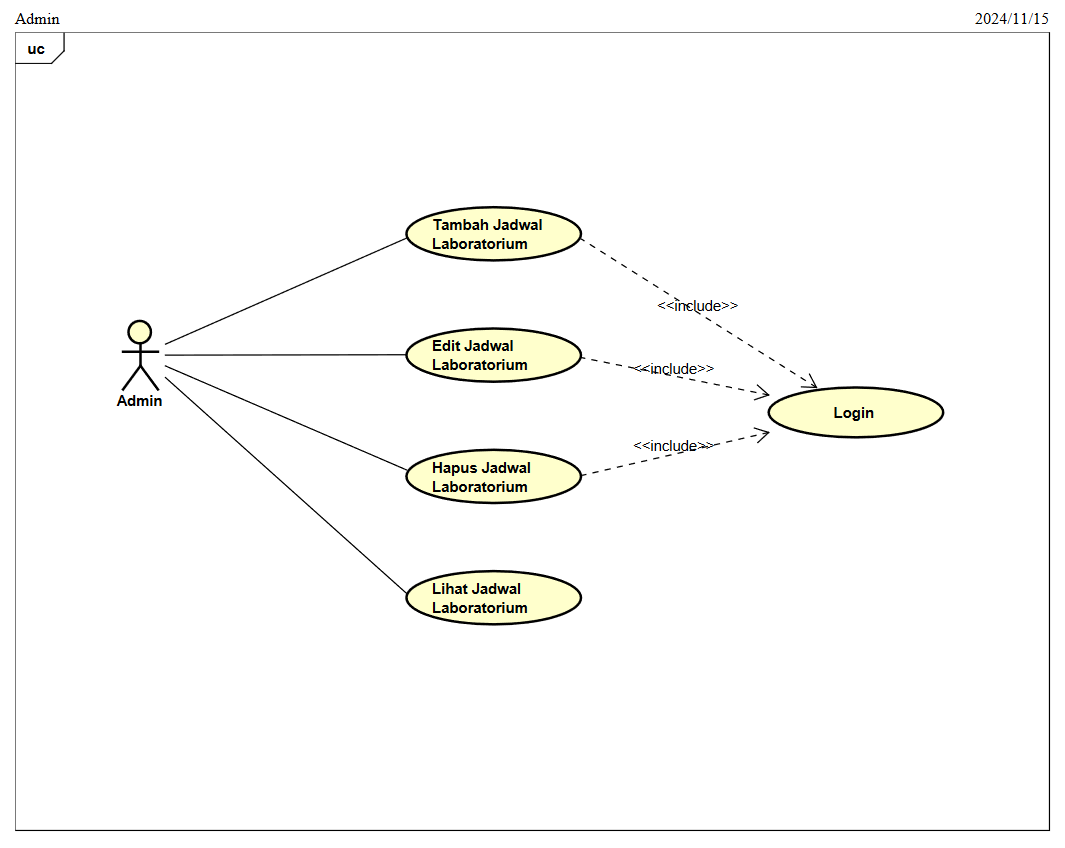
\includegraphics[width=0.82\textwidth]{konten/gambar/usecase-diagram/admin.png}
	\caption{\textit{Usecase Diagram} Admin}
	\label{usecase-diagram-admin}
\end{figure}

Dalam sistem ini, Kalab memiliki empat fungsi utama yang dapat diakses. Fungsi-fungsi tersebut meliputi kemampuan untuk menambahkan jadwal baru melalui fitur "Tambah Jadwal Laboratorium", melakukan perubahan pada jadwal yang sudah ada menggunakan fitur "Edit Jadwal Laboratorium", menghapus jadwal yang tidak diperlukan dengan fitur "Hapus Jadwal Laboratorium", dan melihat seluruh daftar jadwal yang tersedia melalui fitur "Lihat Jadwal Laboratorium".

Keamanan sistem dijamin melalui mekanisme login yang ditunjukkan dengan relasi "include" pada diagram. Tiga fungsi utama, yaitu menambah, mengedit, dan menghapus jadwal, mengharuskan Kalab untuk melakukan login terlebih dahulu sebelum dapat mengakses fungsi-fungsi tersebut. Sementara itu, fungsi untuk melihat jadwal laboratorium dapat diakses secara langsung tanpa perlu melalui proses login terlebih dahulu, seperti yang ditunjukkan pada Gambar \ref{usecase-diagram-kalab}.
\begin{figure}
	\centering
	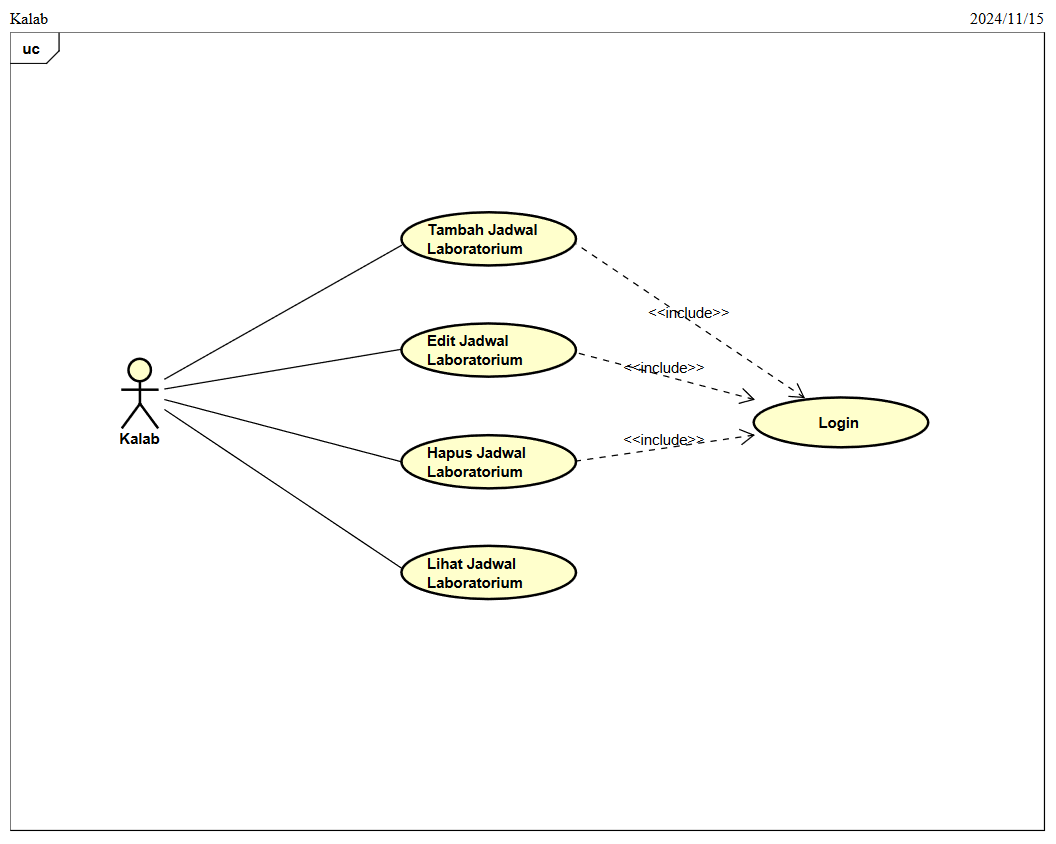
\includegraphics[width=0.82\textwidth]{konten/gambar/usecase-diagram/kalab.png}
	\caption{\textit{Usecase Diagram} Kalab}
	\label{usecase-diagram-kalab}
\end{figure}

Dalam sistem ini, Kaprodi memiliki satu fungsi utama yang dapat diakses, yaitu melihat seluruh daftar jadwal yang tersedia melalui fitur "Lihat Jadwal Laboratorium".

Fungsi ini dapat diakses secara langsung tanpa perlu melalui proses login terlebih dahulu, sehingga Kaprodi dapat dengan mudah memantau jadwal laboratorium yang ada. Hal ini ditunjukkan pada Gambar \ref{usecase-diagram-kaprodi}.
\begin{figure}
	\centering
	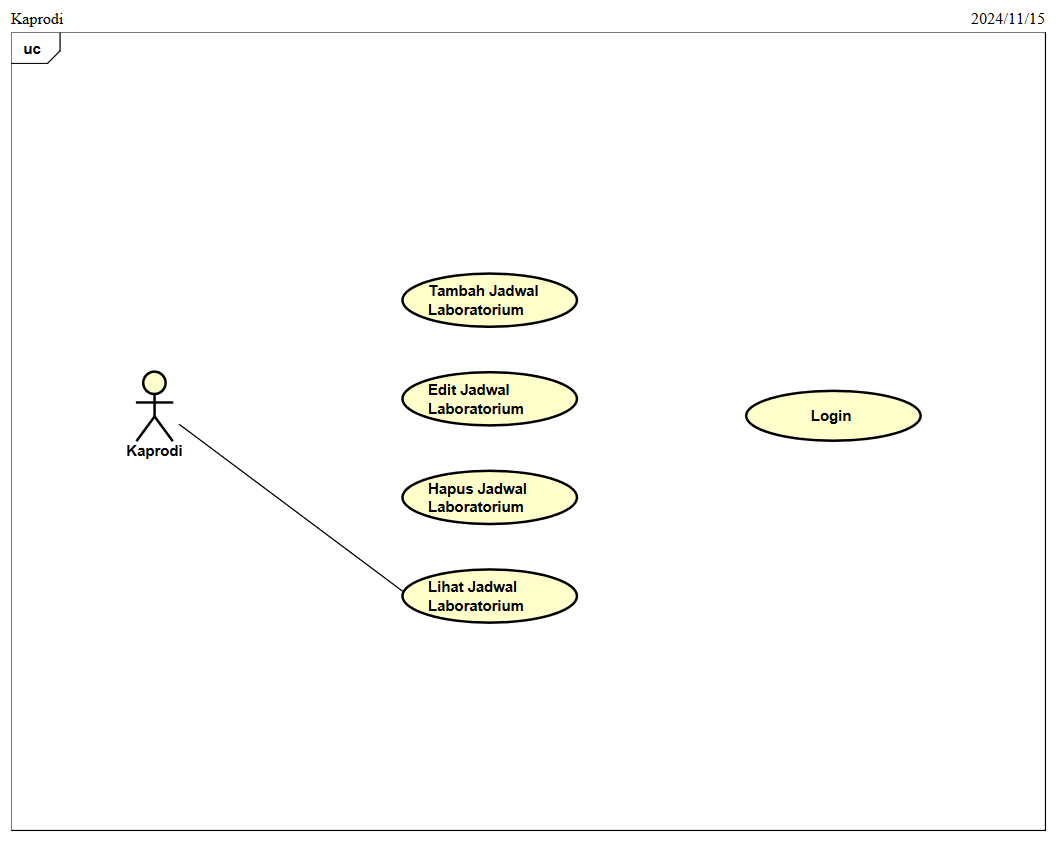
\includegraphics[width=0.82\textwidth]{konten/gambar/usecase-diagram/kaprodi.png}
	\caption{\textit{Usecase Diagram} Kaprodi}
	\label{usecase-diagram-kaprodi}
\end{figure}

Dalam sistem ini, Sekprodi memiliki satu fungsi utama yang dapat diakses, yaitu melihat seluruh daftar jadwal yang tersedia melalui fitur "Lihat Jadwal Laboratorium".

Fungsi ini dapat diakses secara langsung tanpa perlu melalui proses login terlebih dahulu, sehingga Sekprodi dapat dengan mudah memantau jadwal laboratorium yang ada. Hal ini ditunjukkan pada Gambar \ref{usecase-diagram-sekprodi}.
\begin{figure}
	\centering
	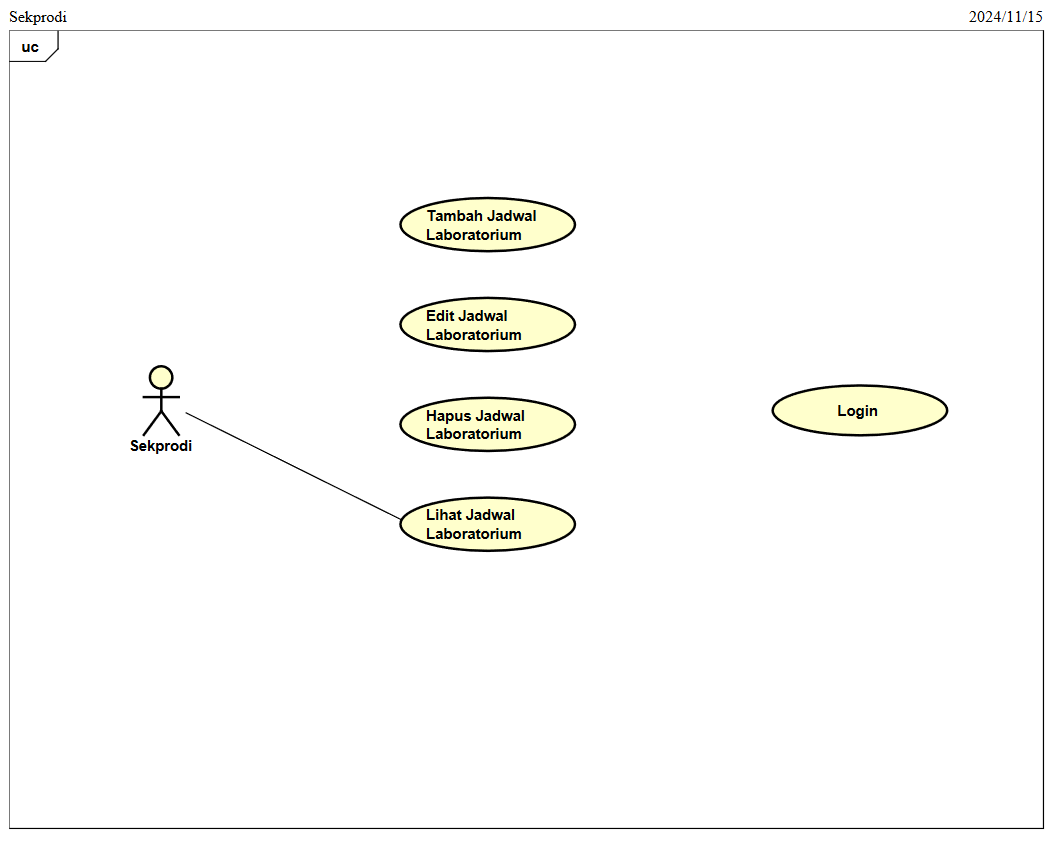
\includegraphics[width=0.82\textwidth]{konten/gambar/usecase-diagram/sekprodi.png}
	\caption{\textit{Usecase Diagram} Sekprodi}
	\label{usecase-diagram-sekprodi}
\end{figure}

Dalam sistem ini, Aslab memiliki empat fungsi utama yang dapat diakses. Fungsi-fungsi tersebut meliputi kemampuan untuk menambahkan jadwal baru melalui fitur "Tambah Jadwal Laboratorium", melakukan perubahan pada jadwal yang sudah ada menggunakan fitur "Edit Jadwal Laboratorium", menghapus jadwal yang tidak diperlukan dengan fitur "Hapus Jadwal Laboratorium", dan melihat seluruh daftar jadwal yang tersedia melalui fitur "Lihat Jadwal Laboratorium".

Keamanan sistem dijamin melalui mekanisme login yang ditunjukkan dengan relasi "include" pada diagram. Tiga fungsi utama, yaitu menambah, mengedit, dan menghapus jadwal, mengharuskan Aslab untuk melakukan login terlebih dahulu sebelum dapat mengakses fungsi-fungsi tersebut. Sementara itu, fungsi untuk melihat jadwal laboratorium dapat diakses secara langsung tanpa perlu melalui proses login terlebih dahulu, seperti yang ditunjukkan pada Gambar \ref{usecase-diagram-kalab}.
\begin{figure}
	\centering
	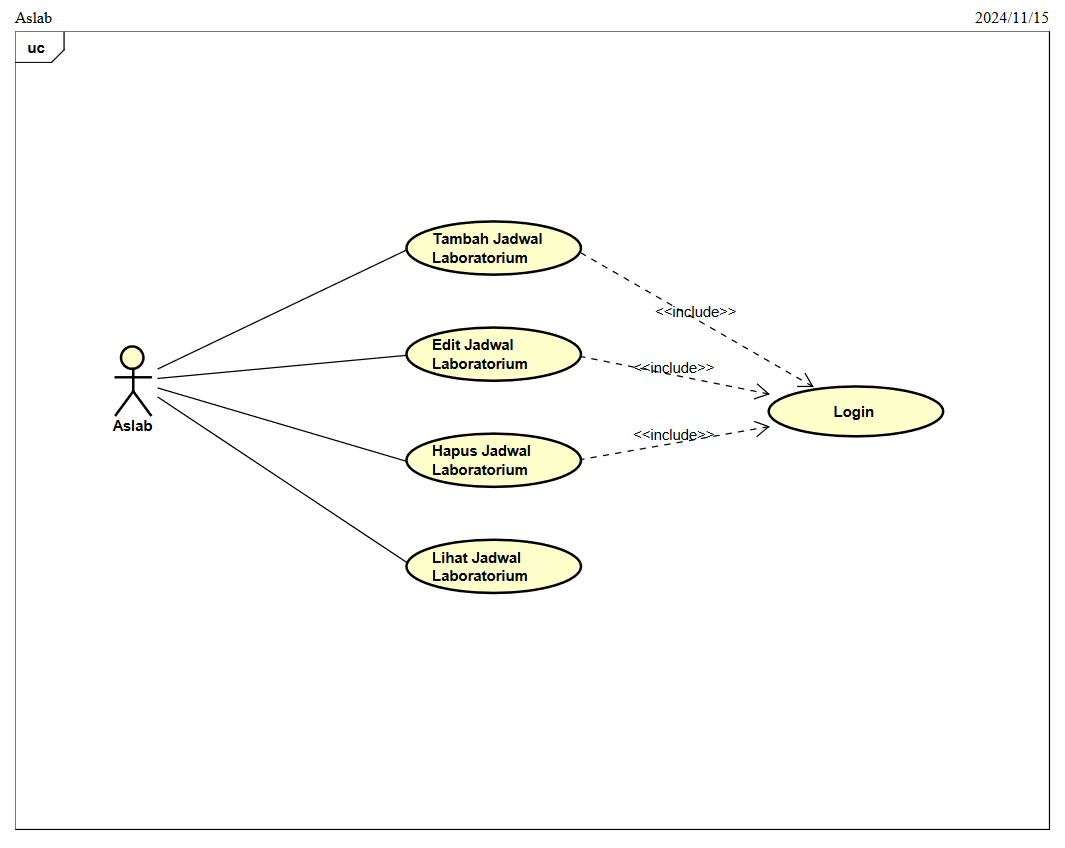
\includegraphics[width=0.82\textwidth]{konten/gambar/usecase-diagram/aslab.png}
	\caption{\textit{Usecase Diagram} Aslab}
	\label{usecase-diagram-aslab}
\end{figure}

% Skenario \textit{use case Login} merujuk pada rangkaian langkah-langkah terstruktur yang harus dilakukan oleh pengguna untuk melakukan proses kegiatan dalam suatu sistem. Proses ini dimulai dengan pengguna yang ingin mengakses sistem harus memasukkan informasi identifikasi pribadi, seperti nim, dan kata sandi, guna memverifikasi identitas mereka. Setelah pengisian data, sistem akan melakukan verifikasi dengan data yang tercatat dalam basis data, dan jika sesuai, pengguna akan diberikan izin akses ke fitur atau informasi yang relevan. Skenario \textit{Use Case Login} memegang peran krusial dalam menjaga tingkat keamanan serta privasi sistem, menjamin bahwa hanya pengguna yang diberi akses yang dapat masuk kedalam sistem.

% Pentingnya tahap ini dalam keamanan sistem ditunjukkan dalam Tabel \ref{tab:SkenarioLogin} yang secara rinci menggambarkan langkah-langkah dalam proses otentikasi. Dengan menjamin kelancaran proses ini, sistem dapat melindungi data sensitif dan memastikan bahwa hanya pengguna yang berwenang yang memiliki akses ke informasi yang terdapat dalam sistem.

% 	{
% 		\fontsize{10}{12}
% 		\begin{longtable}{@{} p{6cm} p{6cm} @{}}
% 			\caption{Skenario \textit{Use Case Login}} \label{tab:SkenarioLogin}                                                                                                                                                                                                           \\ \hline
% 			\textbf{Nama use case}                                                                         & \textit{Login}                                                                                                                                                                \\
% 			\textbf{Aktor}                                                                                 & Admin, Kalab, Aslab, Pendaftar.                                                                                                                                               \\
% 			\textbf{Deskripsi}                                                                             & \textit{Use case} ini menggambarkan untuk dapat mengelola sistem, Admin, Kepala Laboratorium, Pendaftar, Asisten Laboratorium harus melakukan \textit{login} terlebih dahulu. \\
% 			\textbf{Kondisi Awal}                                                                          & Sistem menampilkan form \textit{login}.                                                                                                                                       \\
% 			\textbf{Kondisi Akhir}                                                                         & Sistem menampilkan menu utama.                                                                                                                                                \\ \hline
% 			\multicolumn{1}{c}{\textbf{Aktor}}                                                             & \multicolumn{1}{c}{\textbf{Sistem}}                                                                                                                                           \\ \hline
% 			\multicolumn{2}{c}{\textbf{Skenario normal}}                                                                                                                                                                                                                                   \\ \hline
% 			1. \textit{Use case} ini dimulai ketika Admin, Kalab, Kaprodi, Sekprodi, Aslab \textit{login}. &                                                                                                                                                                               \\
% 			                                                                                               & 2. Sistem melakukan verifikasi \textit{login}.                                                                                                                                \\
% 			                                                                                               & 3. Sistem menampilkan menu utama.                                                                                                                                             \\ \hline
% 			\multicolumn{2}{c}{\textbf{Skenario gagal}}                                                                                                                                                                                                                                    \\ \hline
% 			1. \textit{Use case} ini dimulai ketika Admin, Kalab, Kaprodi, Sekprodi, Aslab \textit{login}. &                                                                                                                                                                               \\
% 			                                                                                               & 2. Sistem melakukan verifikasi \textit{login}.                                                                                                                                \\
% 			                                                                                               & 3. Sistem menampilkan pesan \textit{login} tidak valid.                                                                                                                       \\ \hline
% 		\end{longtable}}

% 	{
% 		\fontsize{10}{12}
% 		\begin{longtable}{@{} p{6cm} p{6cm} @{}}
% 			\caption{Skenario \textit{Use Case Kalab}} \label{tab:SkenarioKalab}                                                                                                                                             \\ \hline
% 			\textbf{Nama use case}                            & \textit{Manajemen Jadwal Laboratorium}                                                                                                                       \\
% 			\textbf{Aktor}                                    & Kalab, Aslab.                                                                                                                                                \\
% 			\textbf{Deskripsi}                                & \textit{Use case} ini menggambarkan proses yang dilakukan oleh Kalab untuk mengelola jadwal laboratorium, termasuk menambah, mengedit, dan menghapus jadwal. \\
% 			\textbf{Kondisi Awal}                             & Sistem menampilkan menu manajemen jadwal.                                                                                                                    \\
% 			\textbf{Kondisi Akhir}                            & Sistem menampilkan daftar jadwal laboratorium yang telah diperbarui.                                                                                         \\ \hline
% 			\multicolumn{1}{c}{\textbf{Aktor}}                & \multicolumn{1}{c}{\textbf{Sistem}}                                                                                                                          \\ \hline
% 			\multicolumn{2}{c}{\textbf{Skenario normal}}                                                                                                                                                                     \\ \hline
% 			1. Kalab memilih opsi untuk menambah jadwal baru. &                                                                                                                                                              \\
% 			                                                  & 2. Sistem menampilkan form untuk input jadwal baru.                                                                                                          \\
% 			                                                  & 3. Kalab mengisi form dan mengirimkan data.                                                                                                                  \\
% 			                                                  & 4. Sistem menyimpan jadwal baru dan menampilkan konfirmasi.                                                                                                  \\ \hline
% 			\multicolumn{2}{c}{\textbf{Skenario gagal}}                                                                                                                                                                      \\ \hline
% 			1. Kalab memilih opsi untuk menambah jadwal baru. &                                                                                                                                                              \\
% 			                                                  & 2. Sistem menampilkan form untuk input jadwal baru.                                                                                                          \\
% 			                                                  & 3. Kalab mengisi form dengan data yang tidak valid.                                                                                                          \\
% 			                                                  & 4. Sistem menampilkan pesan kesalahan dan meminta Kalab untuk memperbaiki data.                                                                              \\ \hline
% 		\end{longtable}}
% 	{

% 		\fontsize{10}{12}
% 		\begin{longtable}{@{} p{6cm} p{6cm} @{}}
% 			\caption{Skenario \textit{Use Case Kalab}} \label{tab:SkenarioKalab}                                                                                                                                             \\ \hline
% 			\textbf{Nama use case}                            & \textit{Manajemen Jadwal Laboratorium}                                                                                                                       \\
% 			\textbf{Aktor}                                    & Kalab, Aslab.                                                                                                                                                \\
% 			\textbf{Deskripsi}                                & \textit{Use case} ini menggambarkan proses yang dilakukan oleh Kalab untuk mengelola jadwal laboratorium, termasuk menambah, mengedit, dan menghapus jadwal. \\
% 			\textbf{Kondisi Awal}                             & Sistem menampilkan menu manajemen jadwal.                                                                                                                    \\
% 			\textbf{Kondisi Akhir}                            & Sistem menampilkan daftar jadwal laboratorium yang telah diperbarui.                                                                                         \\ \hline
% 			\multicolumn{1}{c}{\textbf{Aktor}}                & \multicolumn{1}{c}{\textbf{Sistem}}                                                                                                                          \\ \hline
% 			\multicolumn{2}{c}{\textbf{Skenario normal}}                                                                                                                                                                     \\ \hline
% 			1. Kalab memilih opsi untuk menambah jadwal baru. &                                                                                                                                                              \\
% 			                                                  & 2. Sistem menampilkan form untuk input jadwal baru.                                                                                                          \\
% 			                                                  & 3. Kalab mengisi form dan mengirimkan data.                                                                                                                  \\
% 			                                                  & 4. Sistem menyimpan jadwal baru dan menampilkan konfirmasi.                                                                                                  \\ \hline
% 			\multicolumn{2}{c}{\textbf{Skenario gagal}}                                                                                                                                                                      \\ \hline
% 			1. Kalab memilih opsi untuk menambah jadwal baru. &                                                                                                                                                              \\
% 			                                                  & 2. Sistem menampilkan form untuk input jadwal baru.                                                                                                          \\
% 			                                                  & 3. Kalab mengisi form dengan data yang tidak valid.                                                                                                          \\
% 			                                                  & 4. Sistem menampilkan pesan kesalahan dan meminta Kalab untuk memperbaiki data.                                                                              \\ \hline
% 		\end{longtable}}

% =======================================================================================================================
\subsection{\textit{Activity Diagram}}
\textit{Activity diagram} adalah salah satu alat dalam \textit{Unified Modeling Language} (UML) yang digunakan untuk memvisualisasikan alur kerja atau aktivitas dalam suatu sistem \cite{linzhang2004generating}. Pada sistem ini, \textit{activity diagram} memberikan gambaran rinci tentang proses yang dilalui oleh berbagai aktor seperti Admin, Kalab, Kaprodi, Sekprodi, Aslab.

\textit{Activity diagram} login memberikan gambaran rinci tentang proses login yang dilalui oleh pengguna. Diagram ini memandu langkah-langkah yang terlibat dalam proses login, mulai dari input data oleh pengguna, validasi oleh sistem hingga dapat masuk ke dalam sistem menggunakan akun yang sudah ada. \textit{Activity diagram} ini dapat dilihat pada Gambar \ref{activity-diagram-login}.
\begin{figure}
	\centering
	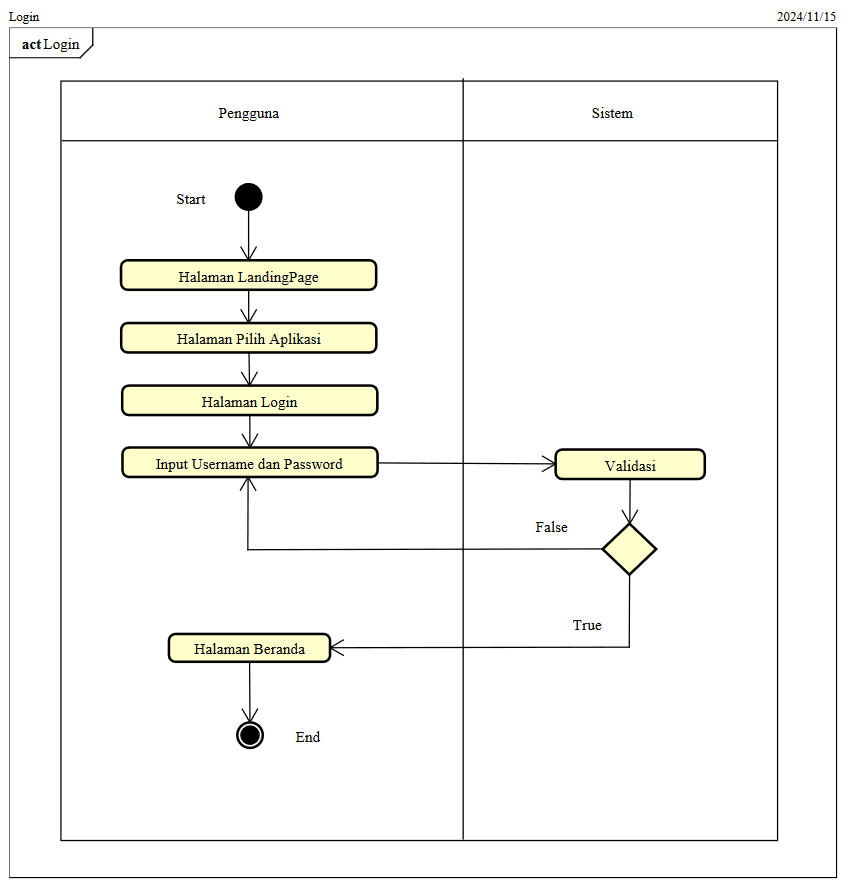
\includegraphics[width=0.82\textwidth]{konten/gambar/activity-diagram/login.png}
	\caption{\textit{Activity Diagram} Login}
	\label{activity-diagram-login}
\end{figure}

\textit{Activity diagram} tambah dosen memberikan gambaran rinci tentang proses penambahan dosen yang dilalui oleh pengguna. Diagram ini memandu langkah-langkah yang terlibat dalam proses penambahan dosen, mulai dari input data oleh pengguna, validasi oleh sistem hingga penyimpanan data dosen baru ke dalam sistem. \textit{Activity diagram} ini dapat dilihat pada Gambar \ref{activity-diagram-tambah-dosen}.
\begin{figure}
	\centering
	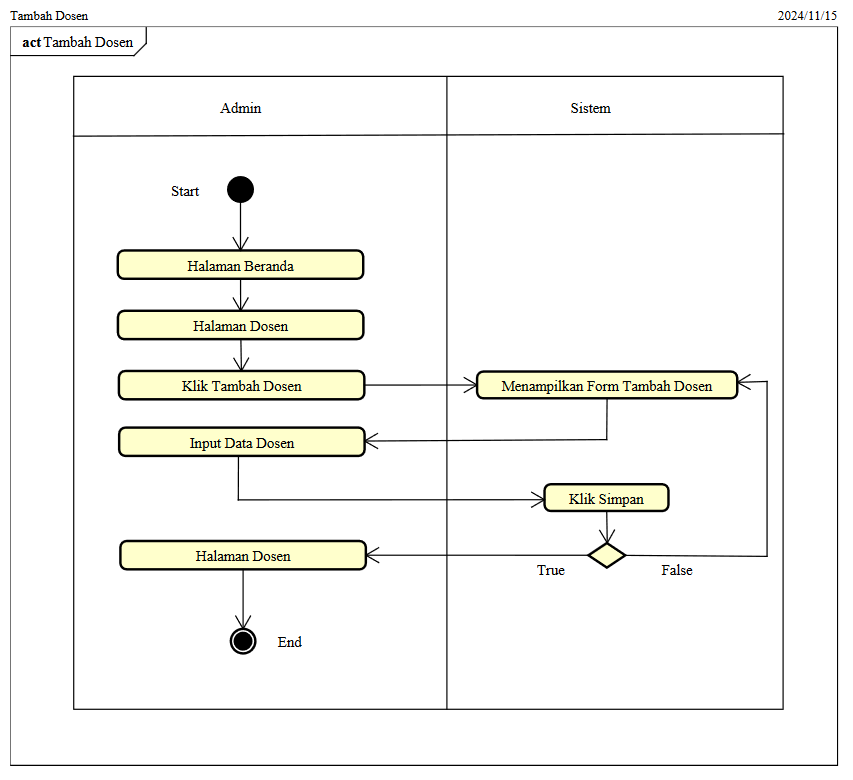
\includegraphics[width=0.82\textwidth]{konten/gambar/activity-diagram/tambah-dosen.png}
	\caption{\textit{Activity Diagram} Tambah Dosen}
	\label{activity-diagram-tambah-dosen}
\end{figure}

\textit{Activity diagram} edit dosen memberikan gambaran rinci tentang proses pengeditan data dosen yang dilalui oleh pengguna. Diagram ini memandu langkah-langkah yang terlibat dalam proses pengeditan dosen, mulai dari pemilihan data dosen yang akan diedit, input data baru oleh pengguna, validasi oleh sistem hingga penyimpanan data dosen yang telah diperbarui ke dalam sistem. \textit{Activity diagram} ini dapat dilihat pada Gambar \ref{activity-diagram-edit-dosen}.
\begin{figure}
	\centering
	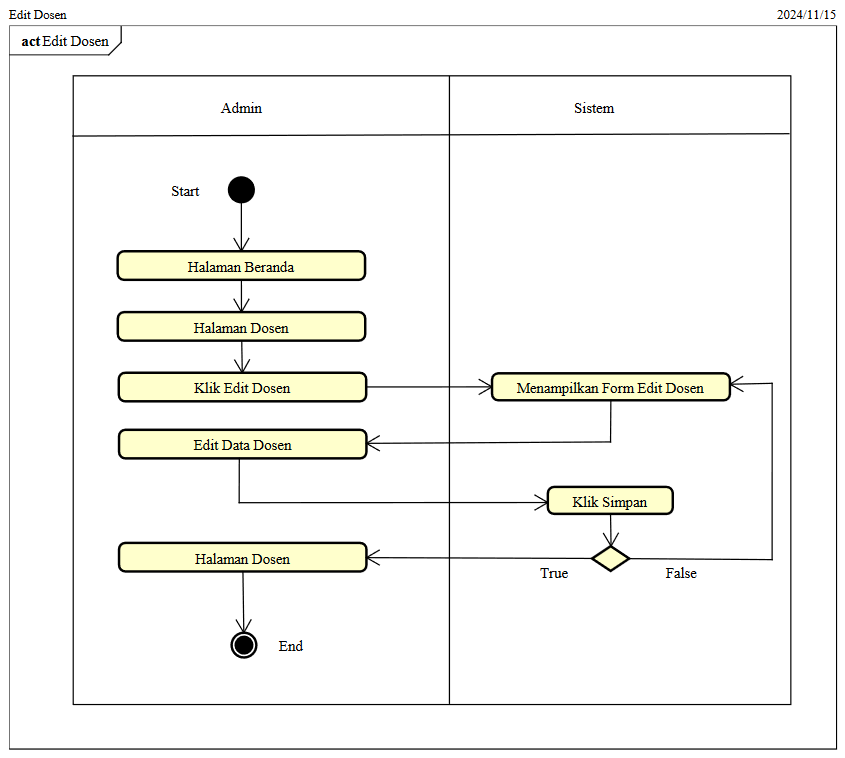
\includegraphics[width=0.82\textwidth]{konten/gambar/activity-diagram/edit-dosen.png}
	\caption{\textit{Activity Diagram} Edit Dosen}
	\label{activity-diagram-edit-dosen}
\end{figure}

\textit{Activity diagram} hapus dosen memberikan gambaran rinci tentang proses penghapusan dosen yang dilalui oleh pengguna. Diagram ini memandu langkah-langkah yang terlibat dalam proses penghapusan dosen, mulai dari pemilihan data dosen yang akan dihapus, konfirmasi oleh pengguna, hingga penghapusan data dosen dari sistem. \textit{Activity diagram} ini dapat dilihat pada Gambar \ref{activity-diagram-hapus-dosen}.
\begin{figure}
	\centering
	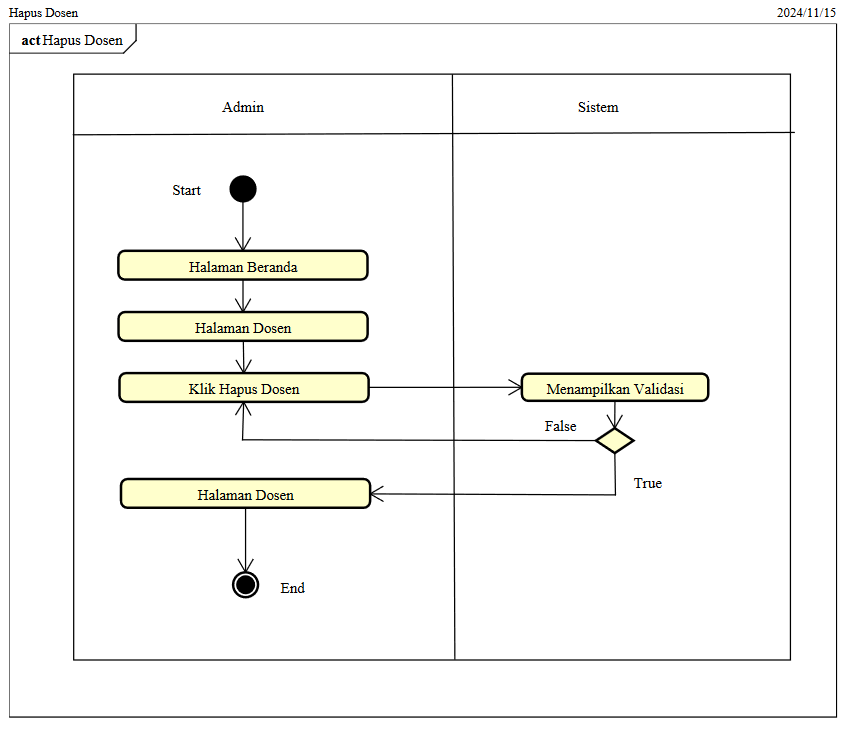
\includegraphics[width=0.82\textwidth]{konten/gambar/activity-diagram/hapus-dosen.png}
	\caption{\textit{Activity Diagram} Hapus Dosen}
	\label{activity-diagram-hapus-dosen}
\end{figure}

\textit{Activity diagram} tambah mata kuliah memberikan gambaran rinci tentang proses penambahan mata kuliah yang dilalui oleh pengguna. Diagram ini memandu langkah-langkah yang terlibat dalam proses penambahan mata kuliah, mulai dari input data oleh pengguna, validasi oleh sistem hingga penyimpanan data mata kuliah baru ke dalam sistem. \textit{Activity diagram} ini dapat dilihat pada Gambar \ref{activity-diagram-tambah-matkul}.
\begin{figure}
	\centering
	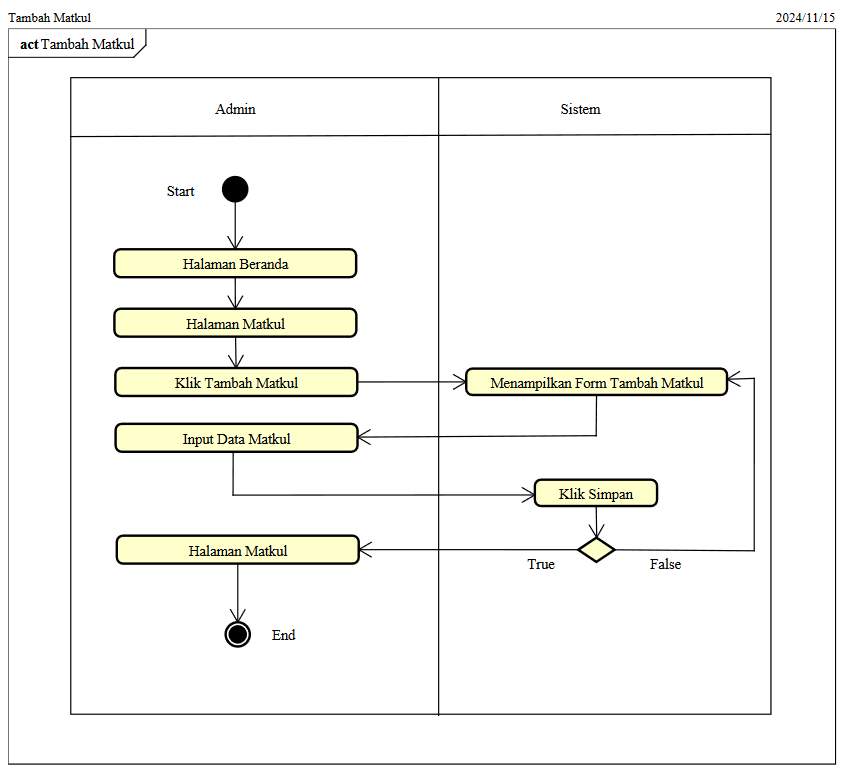
\includegraphics[width=0.82\textwidth]{konten/gambar/activity-diagram/tambah-matkul.png}
	\caption{\textit{Activity Diagram} Tambah Mata Kuliah}
	\label{activity-diagram-tambah-matkul}
\end{figure}

\textit{Activity diagram} edit mata kuliah memberikan gambaran rinci tentang proses pengeditan data mata kuliah yang dilalui oleh pengguna. Diagram ini memandu langkah-langkah yang terlibat dalam proses pengeditan mata kuliah, mulai dari pemilihan data mata kuliah yang akan diedit, input data baru oleh pengguna, validasi oleh sistem hingga penyimpanan data mata kuliah yang telah diperbarui ke dalam sistem. \textit{Activity diagram} ini dapat dilihat pada Gambar \ref{activity-diagram-edit-matkul}.
\begin{figure}
	\centering
	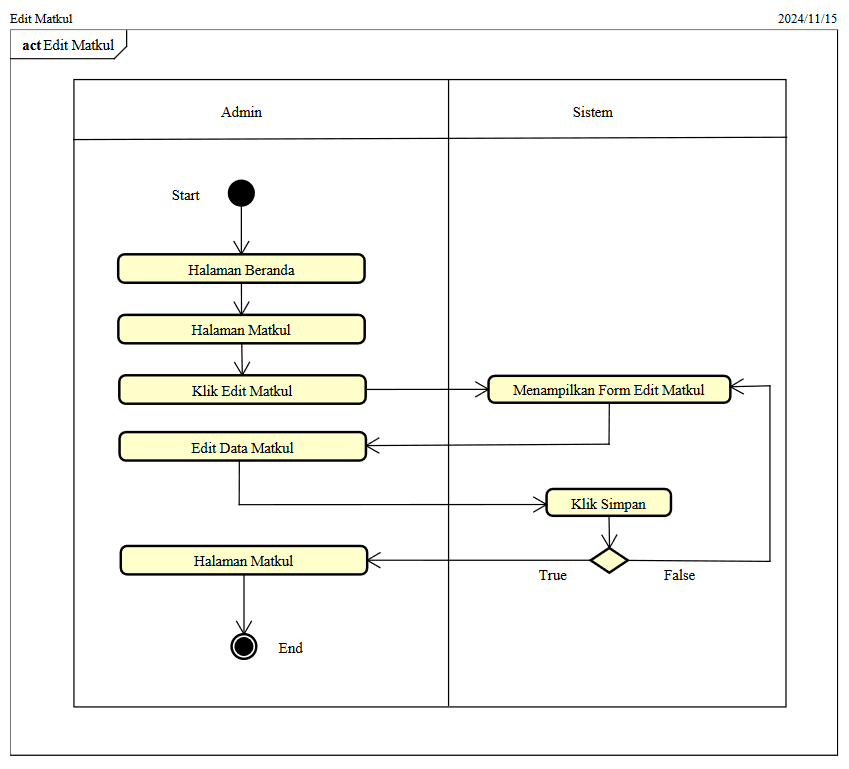
\includegraphics[width=0.82\textwidth]{konten/gambar/activity-diagram/edit-matkul.png}
	\caption{\textit{Activity Diagram} Edit Mata Kuliah}
	\label{activity-diagram-edit-matkul}
\end{figure}

\textit{Activity diagram} hapus mata kuliah memberikan gambaran rinci tentang proses penghapusan mata kuliah yang dilalui oleh pengguna. Diagram ini memandu langkah-langkah yang terlibat dalam proses penghapusan mata kuliah, mulai dari pemilihan data mata kuliah yang akan dihapus, konfirmasi oleh pengguna, hingga penghapusan data mata kuliah dari sistem. \textit{Activity diagram} ini dapat dilihat pada Gambar \ref{activity-diagram-hapus-matkul}.
\begin{figure}
	\centering
	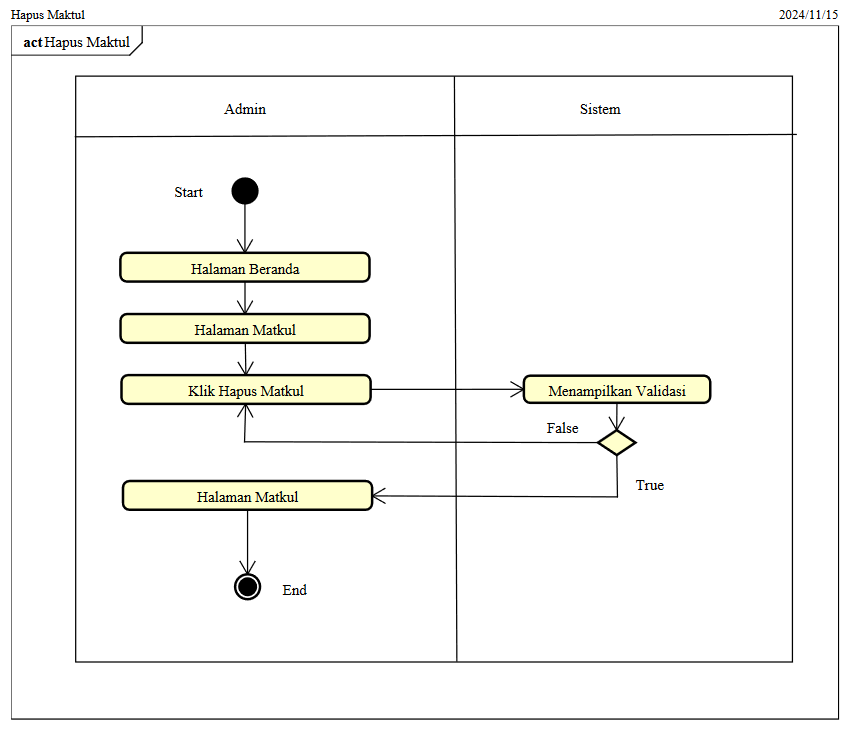
\includegraphics[width=0.82\textwidth]{konten/gambar/activity-diagram/hapus-matkul.png}
	\caption{\textit{Activity Diagram} Hapus Mata Kuliah}
	\label{activity-diagram-hapus-matkul}
\end{figure}

\textit{Activity diagram} tambah dosen memberikan gambaran rinci tentang proses penambahan dosen yang dilalui oleh pengguna. Diagram ini memandu langkah-langkah yang terlibat dalam proses penambahan dosen, mulai dari input data oleh pengguna, validasi oleh sistem hingga penyimpanan data dosen baru ke dalam sistem. \textit{Activity diagram} ini dapat dilihat pada Gambar \ref{activity-diagram-tambah-dosen}.
\begin{figure}
	\centering
	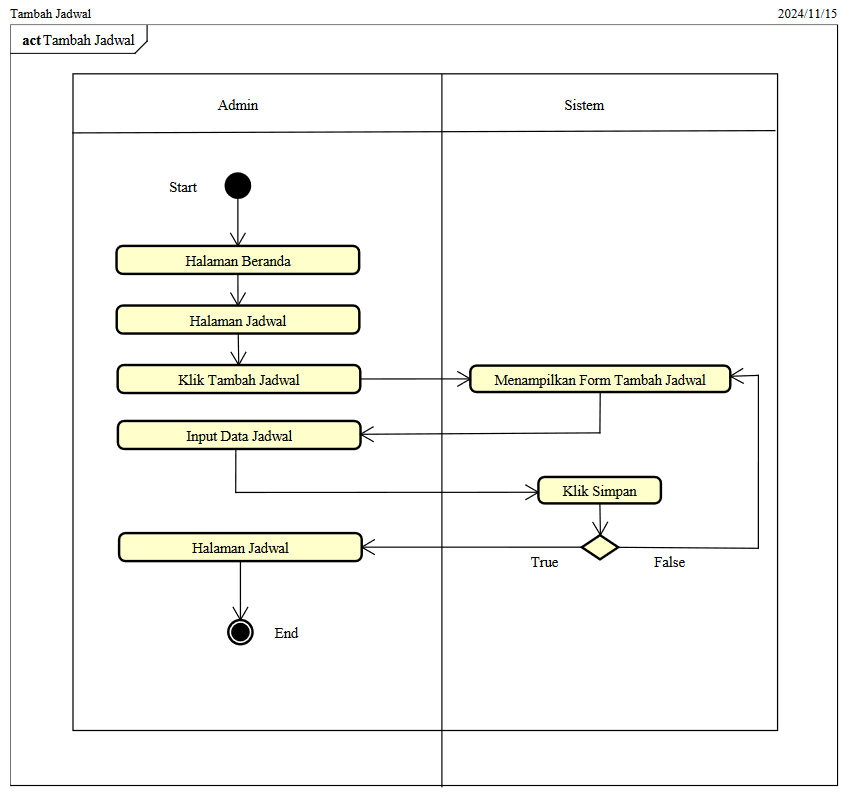
\includegraphics[width=0.82\textwidth]{konten/gambar/activity-diagram/tambah-jadwal.png}
	\caption{\textit{Activity Diagram} Tambah Jadwal}
	\label{activity-diagram-tambah-jadwal}
\end{figure}

\textit{Activity diagram} edit jadwal memberikan gambaran rinci tentang proses pengeditan jadwal yang dilalui oleh pengguna. Diagram ini memandu langkah-langkah yang terlibat dalam proses pengeditan jadwal, mulai dari pemilihan data jadwal yang akan diedit, input data baru oleh pengguna, validasi oleh sistem hingga penyimpanan data jadwal yang telah diperbarui ke dalam sistem. \textit{Activity diagram} ini dapat dilihat pada Gambar \ref{activity-diagram-edit-jadwal}.
\begin{figure}
	\centering
	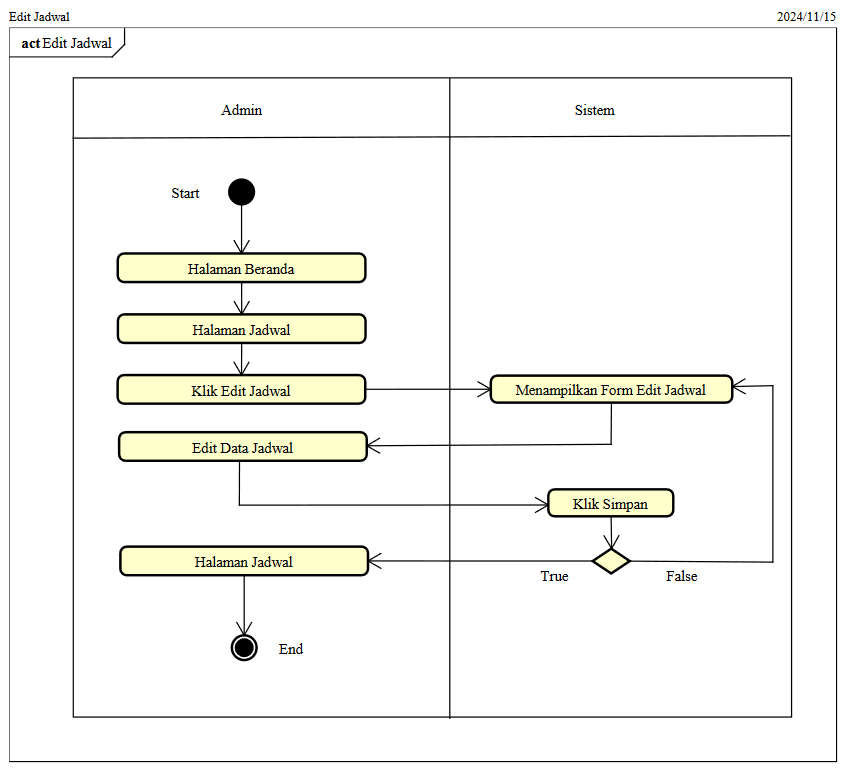
\includegraphics[width=0.82\textwidth]{konten/gambar/activity-diagram/edit-jadwal.png}
	\caption{\textit{Activity Diagram} Edit Jadwal}
	\label{activity-diagram-edit-jadwal}
\end{figure}

\textit{Activity diagram} hapus jadwal memberikan gambaran rinci tentang proses penghapusan jadwal yang dilalui oleh pengguna. Diagram ini memandu langkah-langkah yang terlibat dalam proses penghapusan jadwal, mulai dari pemilihan data jadwal yang akan dihapus, konfirmasi oleh pengguna, hingga penghapusan data jadwal dari sistem. \textit{Activity diagram} ini dapat dilihat pada Gambar \ref{activity-diagram-hapus-jadwal}.
\begin{figure}
	\centering
	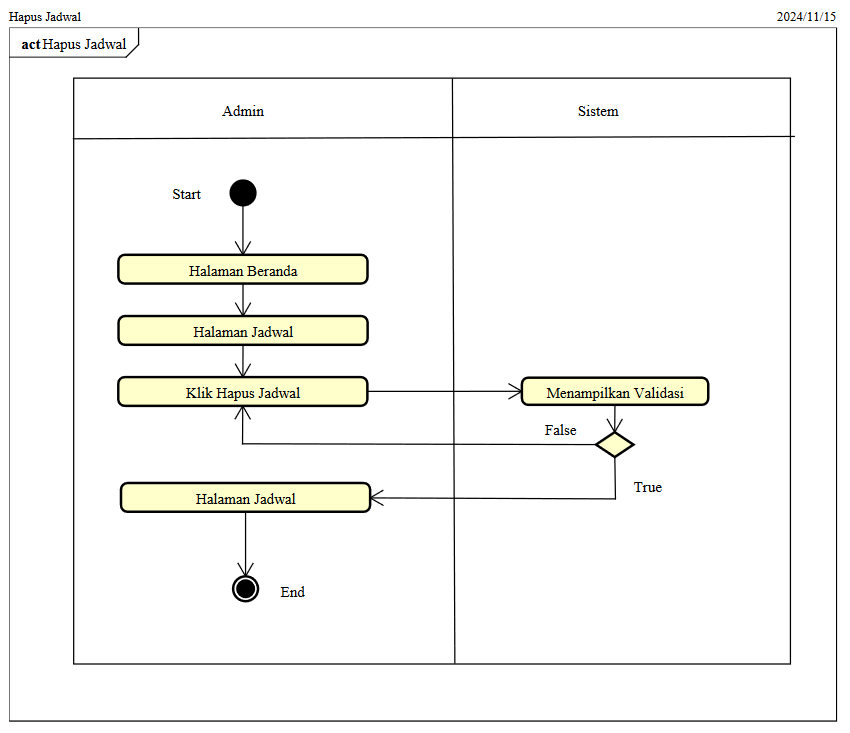
\includegraphics[width=0.82\textwidth]{konten/gambar/activity-diagram/hapus-jadwal.png}
	\caption{\textit{Activity Diagram} Hapus Jadwal}
	\label{activity-diagram-hapus-jadwal}
\end{figure}

% =======================================================================================================================
\subsection{\textit{Class Diagram}}
\textit{Class diagram} adalah representasi visual dari struktur kelas dalam sistem manajemen laboratorium, yang menunjukkan hubungan logis antar kelas. \textit{Class diagram} ini menyediakan deskripsi terperinci dari setiap kelas yang terlibat dalam sistem, termasuk atribut dan operasi yang diperlukan untuk mendukung fungsi manajemen laboratorium secara efektif. \textit{Class diagram} Sistem Informasi Manajemen Laboratorium dapat dilihat pada \pic~\ref{class-diagram}

\begin{figure}
	\centering
	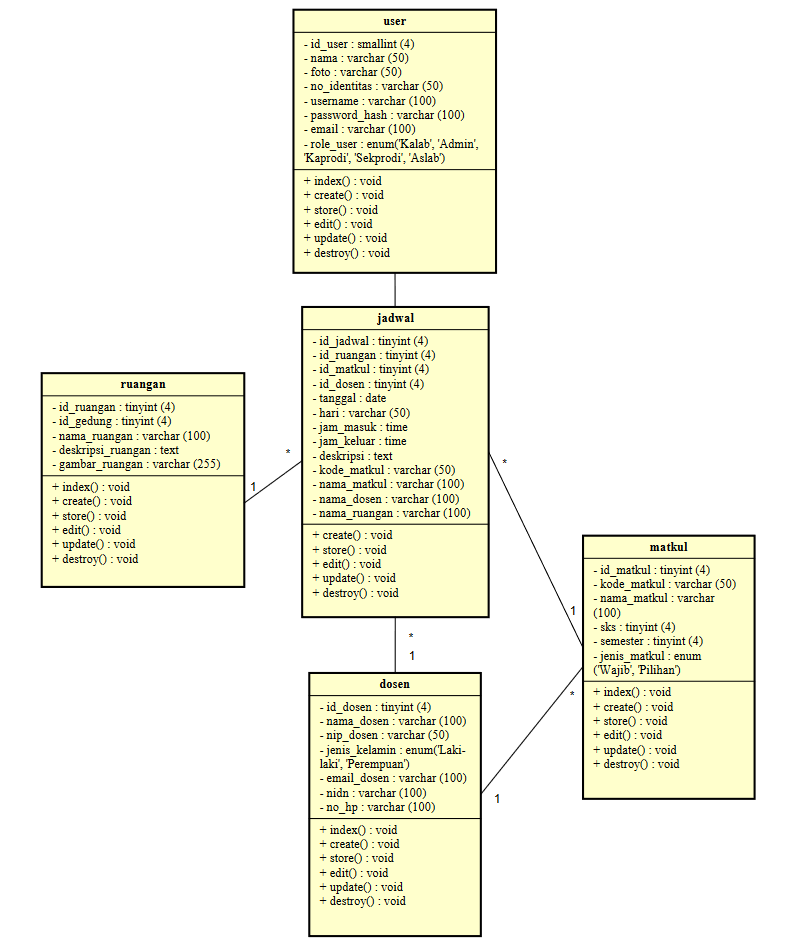
\includegraphics[width=0.82\textwidth]{konten/gambar/class-diagram.png}
	\caption{\textit{Class Diagram} Sistem Manajemen Laboratorium}
	\label{class-diagram}
\end{figure}

Relasi antara jadwal dengan ruangan, dosen, dan mata kuliah diwakili oleh id\_ruangan, id\_dosen, dan id\_matkul pada jadwal. Id\_ruangan menunjukkan keterkaitan jadwal dengan ruangan tertentu, id\_dosen menunjukkan keterkaitan jadwal dengan dosen tertentu, dan id\_matkul menunjukkan keterkaitan jadwal dengan mata kuliah tertentu. Hubungan ini digambarkan dengan garis yang menghubungkan entitas jadwal ke masing-masing entitas ruangan, dosen, dan mata kuliah dalam diagram.

% =======================================================================================================================
\subsection{Perancangan \text{Database}}
Perancangan \textit{database} adalah perancangan basis data yang akan digunakan pada sebuah sistem, didasari oleh data perusahaan. Perancangan ini bertujuan agar tiap field data yang memiliki relasi dapat terhubung pada tabel di \textit{database}, sehingga proses pengaksesan data akan dapat telaksana dengan lebih baik. Berikut adalah detail perancangan serta relasi yang ada pada \textit{database} sistem informasi inventaris laboratorium pada Laboratorium Sistem Informasi. Berikut tabel perancangan \textit{database}:

\begin{enumerate}

	\item Perancangan \textit{Database} Tabel Dosen \\
	      \begin{tabular}{lll}
		      Nama \textit{Database} & : & man\_lab  \\
		      Nama Tabel             & : & dosen     \\
		      Field Kunci            & : & id\_dosen \\
	      \end{tabular}

	      Tabel Dosen dirancang untuk menyimpan informasi komprehensif tentang staf pengajar. Struktur tabel ini mencakup berbagai atribut yang diperlukan untuk mengidentifikasi dan mengelola data dosen secara efisien. Berikut adalah penjelasan ilmiah mengenai struktur dan fungsi tabel Dosen:

	      \begin{itemize}
		      \item Tabel ini menetapkan \textit{id\_dosen} sebagai kunci utama dengan tipe data tinyint(4) dan fitur \textit{auto increment}, yang memastikan bahwa setiap dosen diberikan identifikasi yang unik dalam sistem.
		      \item Atribut 'nama\_dosen' dan 'nip\_dosen' berfungsi untuk menyimpan informasi dasar tentang dosen, yang memudahkan pengenalan personal dalam lingkungan akademis.
		      \item Field 'jenis\_kelamin' memakai tipe data enum untuk menjaga konsistensi data dan membantu dalam analisis demografis.
		      \item 'email\_dosen' dan 'no\_hp' merupakan saluran komunikasi yang vital, yang memungkinkan komunikasi yang efektif antara dosen dan sistem.
		      \item Atribut 'nidn' (Nomor Induk Dosen Nasional) mencatat identifikasi nasional yang unik untuk dosen, yang mendukung integrasi dengan sistem pendidikan tinggi yang lebih luas.
	      \end{itemize}

	      Struktur tabel ini dirancang dengan mempertimbangkan kebutuhan manajemen data dosen yang komprehensif, efisiensi penyimpanan, dan kemudahan dalam pemrosesan dan analisis data.

		      {
			      \fontsize{10}{12}\selectfont
			      \begin{longtable}{l l l l}
				      \caption{Tabel Dosen}
				      \label{admin}                                                                                         \\
				      \hline
				      \textbf{\textit{Field}} & \textbf{\textit{Type}} & \textbf{\textit{Length}}   & \textbf{\textit{Key}} \\
				      \hline
				      \endfirsthead

				      \multicolumn{4}{c}{\tablename\ \thetable\ {Tabel Dosen} \space (Tabel lanjutan...)}                   \\
				      \hline
				      \textbf{\textit{Field}} & \textbf{\textit{Type}} & \textbf{\textit{Length}}   & \textbf{\textit{Key}} \\
				      \hline
				      \endhead

				      id\_dosen               & tinyint                & 4                          & Primary key (A\_I)    \\
				      nama\_dosen             & varchar                & 100                        &                       \\
				      nip\_dosen              & varchar                & 50                         &                       \\
				      jenis\_kelamin          & enum                   & ('Laki-laki', 'Perempuan') &                       \\
				      email\_dosen            & varchar                & 100                        &                       \\
				      nidn                    & varchar                & 100                        &                       \\
				      no\_hp                  & varchar                & 100                        &                       \\
				      \hline
			      \end{longtable}
		      }

	\item Perancangan \textit{Database} Tabel Matkul \\
	      \begin{tabular}{lll}
		      Nama \textit{Database} & : & man\_lab   \\
		      Nama Tabel             & : & matkul     \\
		      Field Kunci            & : & id\_matkul \\
	      \end{tabular}

	      Tabel Matkul dirancang untuk menyimpan informasi tentang mata kuliah yang ditawarkan dalam program akademik. Struktur tabel ini mencakup berbagai atribut yang diperlukan untuk mengidentifikasi dan mengelola data mata kuliah secara efisien. Berikut adalah penjelasan ilmiah mengenai struktur dan fungsi tabel Matkul:

	      \begin{itemize}
		      \item Tabel ini memanfaatkan \textit{id\_matkul} sebagai kunci utama dengan tipe data tinyint(4) dan fitur \textit{auto increment}, yang menjamin bahwa setiap mata kuliah diberi identifikasi yang unik di dalam sistem.
		      \item Atribut 'kode\_matkul' dan 'nama\_matkul' berfungsi untuk menyimpan informasi dasar yang membantu dalam mengenali mata kuliah dengan cepat di lingkungan akademik.
		      \item Field 'sks' dan 'semester' berisi informasi krusial mengenai bobot akademik dan penjadwalan mata kuliah dalam kurikulum, yang penting untuk perencanaan pendidikan.
		      \item Atribut 'jenis\_matkul' memakai tipe data enum untuk membedakan mata kuliah menjadi kategori wajib atau pilihan, mendukung kelancaran dalam pengelolaan kurikulum.
	      \end{itemize}

	      Struktur tabel ini dirancang dengan mempertimbangkan kebutuhan manajemen data mata kuliah yang komprehensif, efisiensi penyimpanan, dan kemudahan dalam pemrosesan dan analisis data kurikulum.

		      {
			      \fontsize{10}{12}\selectfont
			      \begin{longtable}{l l l l}
				      \caption{Tabel Matkul}
				      \label{admin}                                                                                       \\
				      \hline
				      \textbf{\textit{Field}} & \textbf{\textit{Type}} & \textbf{\textit{Length}} & \textbf{\textit{Key}} \\
				      \hline
				      \endfirsthead

				      \multicolumn{4}{c}{\tablename\ \thetable\ {Tabel Matkul} \space (Tabel lanjutan...)}                \\
				      \hline
				      \textbf{\textit{Field}} & \textbf{\textit{Type}} & \textbf{\textit{Length}} & \textbf{\textit{Key}} \\
				      \hline
				      \endhead

				      id\_matkul              & tinyint                & 4                        & Primary key (A\_I)    \\
				      kode\_matkul            & varchar                & 50                       &                       \\
				      nama\_matkul            & varchar                & 100                      &                       \\
				      sks                     & tinyint                & 4                        &                       \\
				      semester                & tinyint                & 4                        &                       \\
				      jenis\_matkul           & enum                   & ('Wajib', 'Pilihan')     &                       \\
				      \hline
			      \end{longtable}
		      }

	\item Perancangan \textit{Database} Tabel Ruangan \\
	      \begin{tabular}{lll}
		      Nama \textit{Database} & : & man\_lab    \\
		      Nama Tabel             & : & ruangan     \\
		      Field Kunci            & : & id\_ruangan \\
	      \end{tabular}

	      Tabel Ruangan dirancang untuk menyimpan informasi tentang ruangan-ruangan yang tersedia untuk kegiatan akademik. Struktur tabel ini mencakup berbagai atribut yang diperlukan untuk mengidentifikasi dan mengelola data ruangan secara efisien. Berikut adalah penjelasan ilmiah mengenai struktur dan fungsi tabel Ruangan:

	      \begin{itemize}
		      \item Tabel ini memanfaatkan \textit{id\_ruangan} sebagai \textit{primary key}. Dengan menggunakan tipe data tinyint(4) dan fitur \textit{auto increment}, tabel ini memastikan bahwa setiap ruangan tercatat dengan identitas uniknya sendiri dalam sistem.
		      \item Atribut 'id\_gedung' bertindak sebagai \textit{foreign key} yang mengaitkan setiap ruangan dengan gedungnya, membantu dalam mengatur lokasi dengan lebih terstruktur.
		      \item Field 'nama\_ruangan' berisi nama yang memudahkan pengguna dalam mengenali setiap ruangan.
		      \item Atribut 'deskripsi\_ruangan' memberikan ruang untuk menambahkan keterangan lebih lanjut mengenai fasilitas atau ciri khas dari ruangan tersebut.
		      \item Field 'gambar\_ruangan' berisi jalur ke file gambar yang berkaitan dengan ruangan, memudahkan dalam visualisasi dan lebih memahami penampilan ruangan tersebut.
	      \end{itemize}

	      Struktur tabel ini dirancang dengan mempertimbangkan kebutuhan manajemen data ruangan yang komprehensif, efisiensi penyimpanan, dan kemudahan dalam pemrosesan dan analisis data fasilitas.

		      {
			      \fontsize{10}{12}\selectfont
			      \begin{longtable}{l l l l}
				      \caption{Tabel Ruangan}
				      \label{admin}                                                                                       \\
				      \hline
				      \textbf{\textit{Field}} & \textbf{\textit{Type}} & \textbf{\textit{Length}} & \textbf{\textit{Key}} \\
				      \hline
				      \endfirsthead

				      \multicolumn{4}{c}{\tablename\ \thetable\ {Tabel Ruangan} \space (Tabel lanjutan...)}               \\
				      \hline
				      \textbf{\textit{Field}} & \textbf{\textit{Type}} & \textbf{\textit{Length}} & \textbf{\textit{Key}} \\
				      \
				      \endhead

				      id\_ruangan             & tinyint                & 4                        & Primary key (A\_I)    \\
				      id\_gedung              & tinyint                & 4                        & Foreign key           \\
				      nama\_ruangan           & varchar                & 100                      &                       \\
				      deskripsi\_ruangan      & text                   &                          &                       \\
				      gambar\_ruangan         & varchar                & 255                      &                       \\
				      \hline
			      \end{longtable}
		      }

	\item Perancangan \textit{Database} Tabel Jadwal \\
	      \begin{tabular}{lll}
		      Nama \textit{Database} & : & man\_lab   \\
		      Nama Tabel             & : & jadwal     \\
		      Field Kunci            & : & id\_jadwal \\
	      \end{tabular}

	      Tabel Jadwal dirancang untuk menyimpan informasi tentang penjadwalan kegiatan akademik. Struktur tabel ini mencakup berbagai atribut yang diperlukan untuk mengidentifikasi dan mengelola data jadwal secara efisien. Berikut adalah penjelasan ilmiah mengenai struktur dan fungsi tabel Jadwal:

	      \begin{itemize}
		      \item Tabel ini dilengkapi dengan \textit{id\_jadwal} sebagai \textit{primary key}. Dengan tipe data tinyint(4) dan fitur \textit{auto increment}, setiap jadwal dijamin memiliki identifikasi yang unik dalam sistem.
		      \item Atribut seperti 'id\_ruangan', 'id\_matkul', dan 'id\_dosen' bertindak sebagai \textit{foreign key}, yang mengaitkan jadwal dengan informasi tentang ruangan, mata kuliah, dan dosen yang relevan, sehingga memudahkan pengelolaan jadwal secara terpadu.
		      \item Field seperti 'tanggal', 'hari', 'jam\_masuk', dan 'jam\_keluar' berperan penting dalam mencatat waktu spesifik untuk setiap kegiatan dalam jadwal.
		      \item Atribut 'deskripsi' memberikan ruang untuk menambahkan informasi detail tentang kegiatan atau jadwal yang direncanakan.
		      \item Field-field seperti 'kode\_matkul', 'nama\_matkul', 'nama\_dosen', dan 'nama\_ruangan' walaupun redundan, tetapi sangat membantu dalam mempercepat akses informasi tanpa perlu menggabungkan tabel berulang kali.
	      \end{itemize}

	      Struktur tabel ini dirancang dengan mempertimbangkan kebutuhan manajemen data jadwal yang komprehensif, efisiensi dalam pengambilan data, dan fleksibilitas dalam pengelolaan jadwal akademik.

		      {
			      \fontsize{10}{12}\selectfont
			      \begin{longtable}{l l l l}
				      \caption{Tabel Jadwal}
				      \label{admin}                                                                                       \\
				      \hline
				      \textbf{\textit{Field}} & \textbf{\textit{Type}} & \textbf{\textit{Length}} & \textbf{\textit{Key}} \\
				      \hline
				      \endfirsthead

				      \multicolumn{4}{c}{\tablename\ \thetable\ {Tabel Jadwal} \space (Tabel lanjutan...)}                \\
				      \hline
				      \textbf{\textit{Field}} & \textbf{\textit{Type}} & \textbf{\textit{Length}} & \textbf{\textit{Key}} \\
				      \hline
				      \endhead

				      id\_jadwal              & tinyint                & 4                        & Primary key (A\_I)    \\
				      id\_ruangan             & tinyint                & 4                        & Foreign key           \\
				      id\_matkul              & varchar                & 4                        & Foreign key           \\
				      id\_dosen               & varchar                & 4                        & Foreign key           \\
				      tanggal                 & date                   &                          &                       \\
				      hari                    & varchar                & 50                       &                       \\
				      jam\_masuk              & time                   &                          &                       \\
				      jam\_keluar             & time                   &                          &                       \\
				      deskripsi               & text                   &                          &                       \\
				      kode\_matkul            & tinyint                & 4                        &                       \\
				      nama\_matkul            & varchar                & 100                      &                       \\
				      nama\_dosen             & varchar                & 100                      &                       \\
				      nama\_ruangan           & varchar                & 100                      &                       \\
				      \hline
			      \end{longtable}
		      }

	\item Perancangan \textit{Database} Tabel \textit{User} \\
	      \begin{tabular}{lll}
		      Nama \textit{Database} & : & man\_lab          \\
		      Nama Tabel             & : & \textit{user}     \\
		      Field Kunci            & : & id\_\textit{user} \\
	      \end{tabular}

	      Tabel \textit{User} dirancang untuk menyimpan informasi pengguna dalam sistem manajemen laboratorium. Struktur tabel ini mencakup berbagai atribut yang diperlukan untuk mengidentifikasi dan mengautentikasi pengguna, serta mengelola hak akses mereka. Berikut adalah penjelasan ilmiah mengenai struktur dan fungsi tabel \textit{User}:

	      \begin{itemize}
		      \item Tabel ini memberikan setiap pengguna identifikasi unik melalui \textit{id\_user} yang bertindak sebagai \textit{primary key}. Tipe data yang digunakan adalah smallint(4) dengan fitur \textit{auto increment}.
		      \item Atribut 'nama' dan 'no\_identitas' berfungsi untuk menyimpan informasi dasar tentang pengguna, sehingga memudahkan pengenalan personal dalam lingkup organisasi.
		      \item Field 'foto' berisi lokasi penyimpanan file gambar profil pengguna, yang membantu dalam personalisasi tampilan antarmuka pengguna.
		      \item \textit{Username} dan \textit{password\_hash} digunakan sebagai kredensial untuk masuk ke sistem, dengan \textit{password} yang telah dienkripsi guna menjaga keamanan data.
		      \item Atribut 'role\_user' dengan tipe data enum digunakan untuk menentukan peran pengguna dalam sistem, yang mendukung pengelolaan hak akses secara efektif.
	      \end{itemize}

	      Struktur tabel ini dirancang dengan mempertimbangkan aspek keamanan, efisiensi penyimpanan data, dan fleksibilitas dalam pengelolaan pengguna sistem.

		      {
			      \fontsize{10}{12}\selectfont
			      \begin{longtable}{l l l l}
				      \caption{Tabel \textit{User}}
				      \label{admin}                                                                                                                 \\
				      \hline
				      \textbf{\textit{Field}} & \textbf{\textit{Type}} & \textbf{\textit{Length}}                           & \textbf{\textit{Key}} \\
				      \hline
				      \endfirsthead

				      \multicolumn{4}{c}{\tablename\ \thetable\ {Tabel \textit{User}} \space (Tabel lanjutan...)}                                   \\
				      \hline
				      \textbf{\textit{Field}} & \textbf{\textit{Type}} & \textbf{\textit{Length}}                           & \textbf{\textit{Key}} \\
				      \hline
				      \endhead

				      id\_\textit{user}       & smallint               & 4                                                  & Primary key (A\_I)    \\
				      nama                    & varchar                & 50                                                 &                       \\
				      foto                    & varchar                & 50                                                 &                       \\
				      no\_identitas           & varchar                & 50                                                 &                       \\
				      \textit{username}       & varchar                & 100                                                &                       \\
				      \textit{password}\_hash & varchar                & 100                                                &                       \\
				      role\_\textit{user}     & enum                   & ('Admin', 'Kalab', 'Kaprodi', 'Sekprodi', 'Aslab') &                       \\
				      \hline
			      \end{longtable}
		      }

\end{enumerate}

% =======================================================================================================================
\subsection{Perancangan Struktur Menu}
Perancangan menu sistem informasi manajemen inventaris laboratorium dibagi menjadi 5 tingkatan hak akses sesuai kewenangan pengguna. Setiap pengguna dapat mengakses fitur sesuai peran dan tanggung jawab mereka.

Menu Admin, sebagai tingkat akses tertinggi, memiliki wewenang penuh untuk mengelola semua fitur, termasuk pendanaan, manajemen barang, penjadwalan, dll. Kepala Laboratorium (Kalab) memiliki akses hampir sama dengan Admin, tetapi dengan beberapa pembatasan. Kalab dapat mengelola pendanaan, barang, jadwal, dan data dosen serta mata kuliah. Ketua Program Studi (Kaprodi) dan Sekretaris Program Studi (Sekprodi) fokus pada pengawasan dan monitoring, dengan akses ke fitur pendanaan, manajemen barang, dan dokumentasi. Asisten Laboratorium (Aslab) memiliki akses untuk mendukung operasional harian termasuk pengelolaan barang, dan pemeliharaan peralatan laboratorium.

Struktur menu yang terorganisir ini dirancang untuk memudahkan pengelolaan inventaris laboratorium secara sistematis dan terkontrol. Setiap tingkatan pengguna memiliki batasan akses yang jelas, yang membantu dalam menjaga keamanan dan integritas data sistem. Perancangan menu ini menjadi landasan penting dalam pengembangan antarmuka pengguna dan implementasi berbagai fungsi sistem yang akan dibahas lebih lanjut pada bagian berikutnya. Dengan struktur menu yang terorganisir ini, diharapkan pengelolaan inventaris laboratorium dapat berjalan lebih efisien dan terkoordinasi dengan baik antar berbagai tingkatan pengguna. Gambar struktur menu ini dapat dilihat pada \pic~\ref{StrukturMenuILMIS}

\begin{figure}
	\centering
	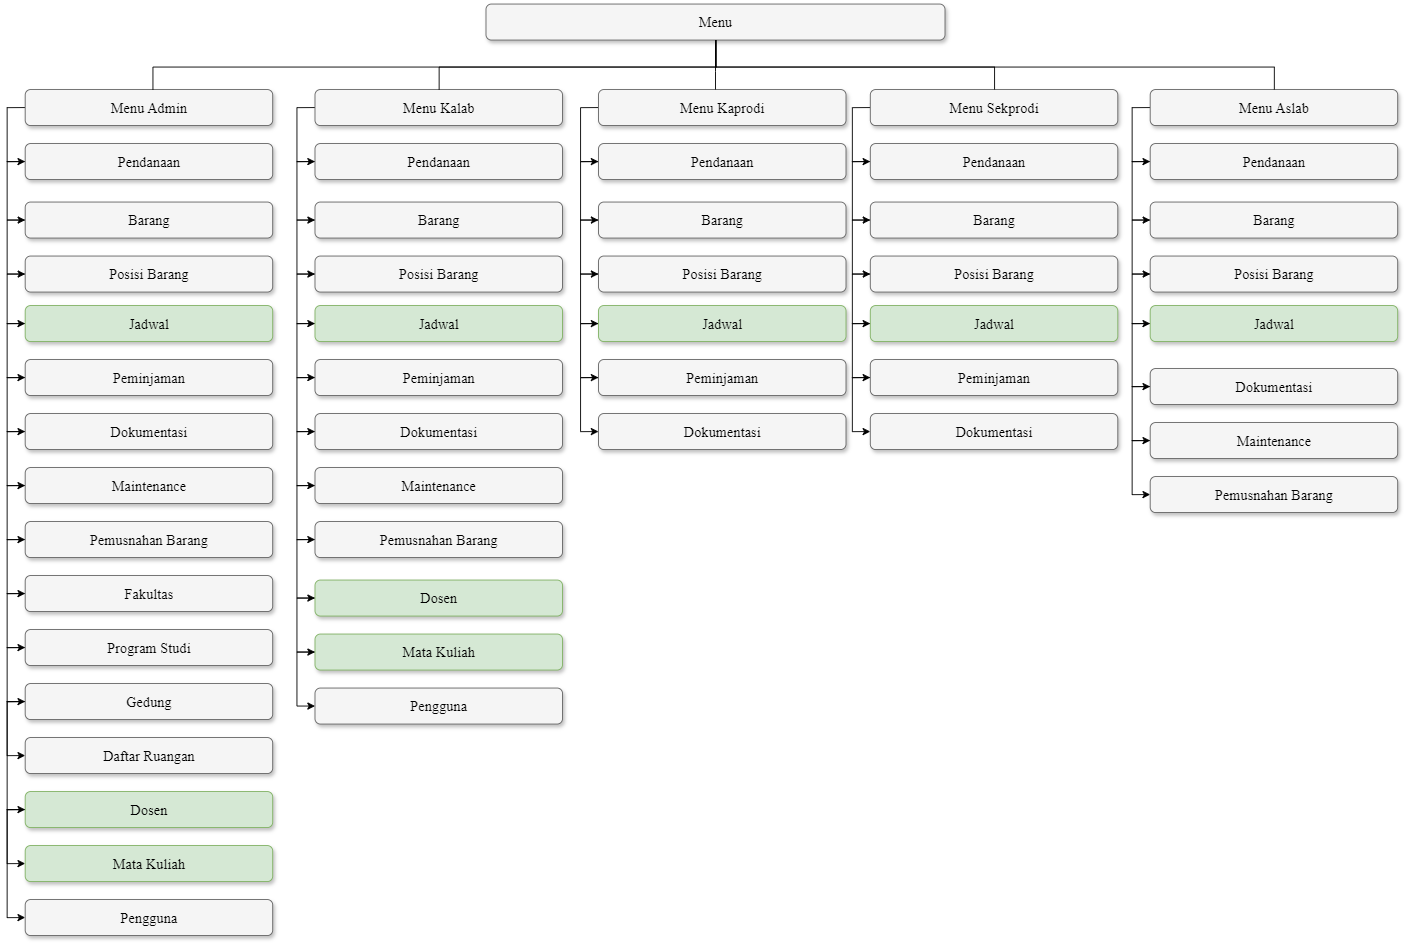
\includegraphics[width=0.82\textwidth]{konten/gambar/menu.png}
	\caption{Struktur Menu Sistem Manajemen Laboratorium}
	\label{StrukturMenuILMIS}
\end{figure}

Pengembangan sistem ini menambahkan fitur baru yang ditandai dengan warna hijau pada struktur menu, termasuk fitur Jadwal untuk semua level pengguna (Admin, Kalab, Kaprodi, Sekprodi, dan Aslab) serta fitur Dosen dan Mata Kuliah yang kini dapat diakses oleh Kalab. Penambahan ini bertujuan untuk meningkatkan pengelolaan laboratorium dan efisiensi koordinasi antara pengelola dan dosen.

% =======================================================================================================================
\subsection{Perancangan \textit{Interface}}
Perancangan \textit{interface} berfungsi untuk menjelaskan tentang desain program sistem informasi manajemen laboratorium yang akan dibangun. Hal ini dilakukan untuk mempermudah pengguna dalam mengetahui proses yang terdapat pada sistem informasi manajemen laboratorium tersebut.

\begin{enumerate}
	\item Rancangan tampilan \textit{landing page} yang berfungsi sebagai halaman pertama untuk sistem informasi manajemen laboratorium dapat dilihat pada \pic~\ref{fig:kelola-jadwal-1}
	      \begin{figure}
		      \centering
		      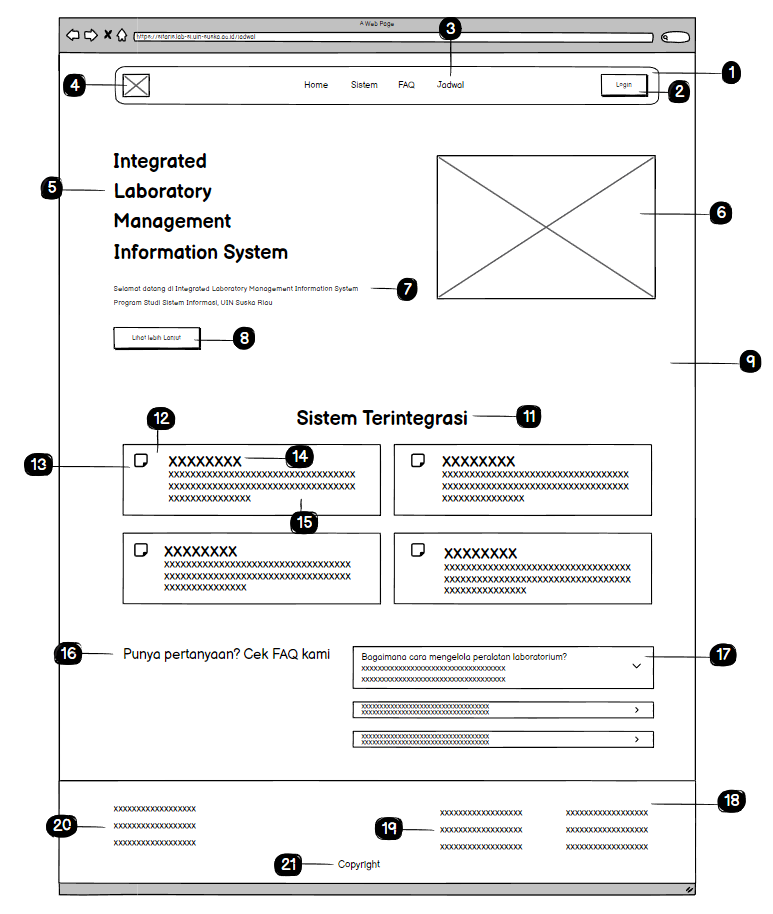
\includegraphics[width=0.82\textwidth]{konten/gambar/landing-page.png}
		      \caption{Tampilan Halaman Utama Sistem Manajemen Laboratorium}
		      \label{fig:kelola-jadwal-1}
	      \end{figure}

	      \begin{longtable}{|c|p{0.55\textwidth}|}
		      \caption{Tabel Keterangan Tampilan Halaman Utama Sistem Manajemen Laboratorium}                                                                 \\
		      \hline
		      \textbf{Nomor Callouts} & \textbf{Keterangan}                                                                                                   \\
		      \hline
		      \endfirsthead

		      \multicolumn{2}{c}{{\textit{Lanjutan dari halaman sebelumnya...}}}                                                                              \\
		      \hline
		      \textbf{Nomor Callouts} & \textbf{Keterangan}                                                                                                   \\
		      \hline
		      \endhead

		      \hline \multicolumn{2}{|r|}{{\textit{Bersambung ke halaman berikutnya...}}}                                                                     \\
		      \endfoot

		      \hline
		      \endlastfoot

		      1                       & Browser toolbar dengan width: 100\%, height: 40px, background-color: \#FFFFFF                                         \\
		      2                       & Logo berukuran width: 40px, height: 40px, dengan margin-left: 24px pada pojok kiri atas                               \\
		      3                       & Navigation menu menggunakan font-family: Poppins, font-size: 14px, dengan gap: 32px antar menu                        \\
		      4                       & Button Login dengan padding: 8px 16px, border-radius: 6px, background-color: \#2563EB                                 \\
		      5                       & Container header dengan width: 100\%, height: 64px, box-shadow: 0 1px 3px rgba(0,0,0,0.1)                             \\
		      6                       & Text "Integrated Laboratory" menggunakan font-family: Poppins, font-size: 48px, font-weight: 600, margin-bottom: 16px \\
		      7                       & Text "Management Information System" berwarna \#2563EB dengan font-weight: 600                                        \\
		      8                       & Button "Lihat Lebih Lanjut" dengan padding: 12px 24px, background-color: \#2563EB                                     \\
		      9                       & Container image dengan width: 560px, height: 400px, border-radius: 8px                                                \\
		      10                      & Container content dengan max-width: 560px dan margin-right: 64px                                                      \\
		      11                      & Heading "Sistem Terintegrasi" dengan text-align: center, font-size: 36px, margin: 64px 0 32px                         \\
		      12                      & Container cards dengan display: grid, grid-template-columns: repeat(2, 1fr), gap: 24px                                \\
		      13                      & Card pertama dengan padding: 24px, background: white, border-radius: 8px, box-shadow: 0 1px 3px rgba(0,0,0,0.1)       \\
		      14                      & Text content pada card dengan font-size: 14px, line-height: 1.6, color: \#374151                                      \\
		      15                      & Card kedua dengan styling sama seperti card pertama                                                                   \\
		      16                      & Card ketiga dengan styling sama seperti card pertama                                                                  \\
		      17                      & Section FAQ dengan max-width: 800px, margin: 64px auto                                                                \\
		      18                      & Container question dengan padding: 24px, border-bottom: 1px solid \#E5E7EB                                            \\
		      19                      & Footer section dengan background: \#1E293B, padding: 64px 24px                                                        \\
		      20                      & Copyright text dengan font-size: 14px, color: \#9CA3AF                                                                \\
		      21                      & Footer links dengan display: flex, gap: 32px, margin-top: 32px                                                        \\
	      \end{longtable}

	\item Rancangan tampilan pilih aplikasi untuk login dapat dilihat pada \pic~\ref{fig:kelola-jadwal-2}
	      \begin{figure}
		      \centering
		      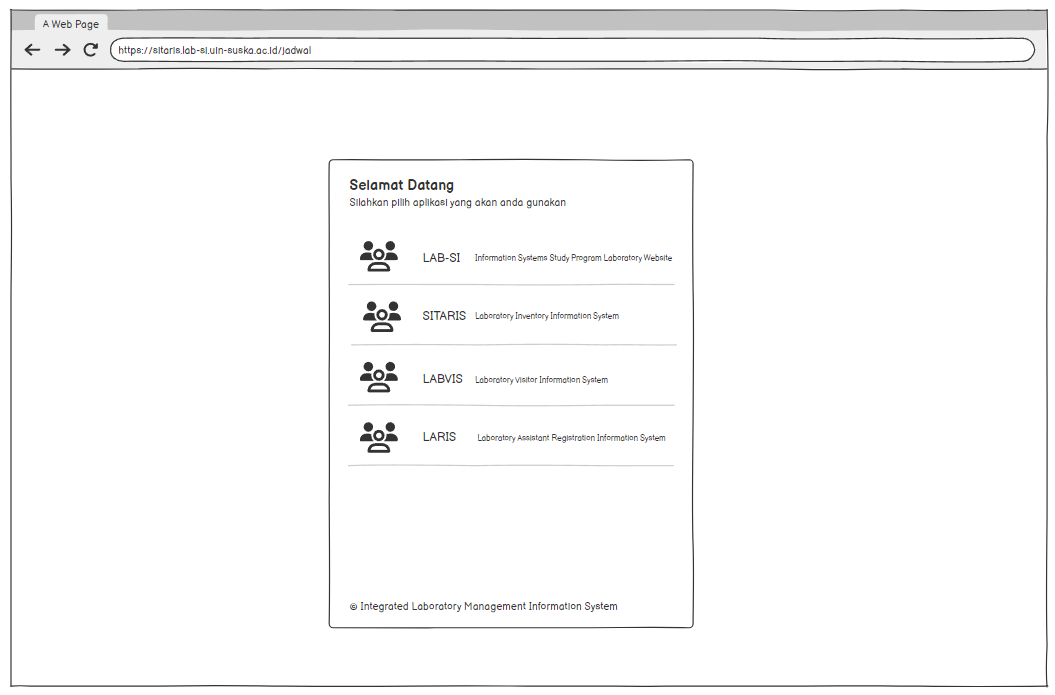
\includegraphics[width=0.82\textwidth]{konten/gambar/pilih-login.png}
		      \caption{Tampilan Pilihan Login untuk Sistem Manajemen Laboratorium}
		      \label{fig:kelola-jadwal-2}
	      \end{figure}

	      \begin{table}[H]
		      \centering
		      \caption{Tabel Keterangan Tampilan Halaman Selamat Datang}
		      \begin{tabular}{|c|p{0.55\textwidth}|}
			      \hline
			      \textbf{Nomor Callouts} & \textbf{Keterangan}                                                                          \\
			      \hline
			      1                       & Text header "Selamat Datang" dengan fonts Poppins, warna font \#73879C                       \\
			      2                       & Text sub-header "Silahkan pilih aplikasi yang akan anda gunakan" dengan fonts Helvetica Neue \\
			      3                       & Container card dengan background color \#FFFFFF dan border-radius 8px                        \\
			      4                       & Link ILMIS dengan icon users dan text "Integrated Laboratory Management Information System"  \\
			      5                       & Link LABVIS dengan icon users dan text "Laboratory Visitor Information System"               \\
			      6                       & Link LARIS dengan icon users dan text "Laboratory Assistant Registration Information System" \\
			      \hline
		      \end{tabular}
	      \end{table}

	\item Rancangan tampilan kelola jadwal yang berfungsi untuk mengelola jadwal laboratorium dapat dilihat pada \pic~\ref{fig:jadwal}
	      \begin{figure}
		      \centering
		      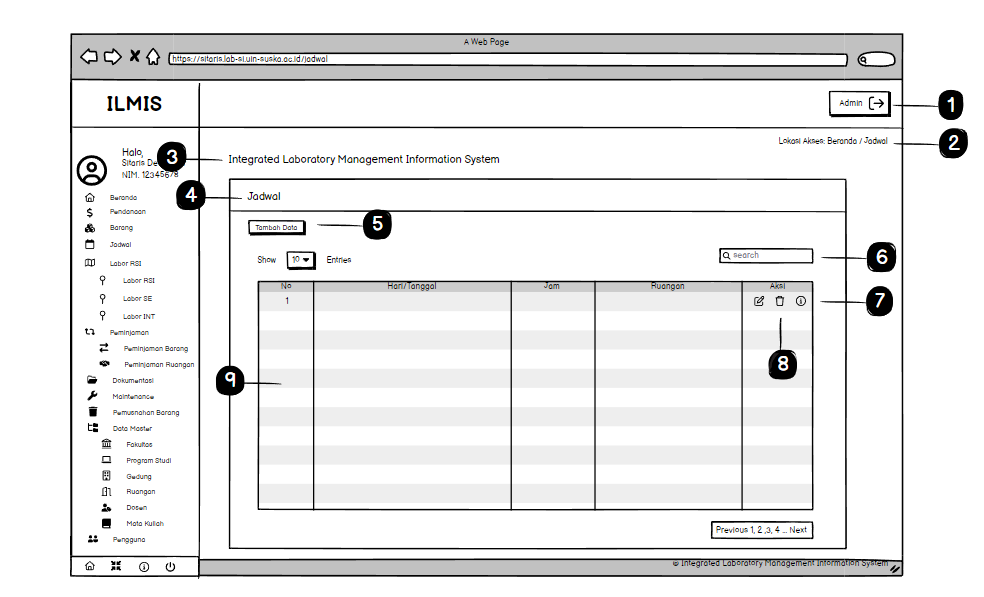
\includegraphics[width=0.82\textwidth]{konten/gambar/user interface/ui-jadwal.png}
		      \caption{Tampilan Kelola Jadwal Laboratorium}
		      \label{fig:jadwal}
	      \end{figure}

	      \begin{table}[H]
		      \centering
		      \caption{Tabel Keterangan Tampilan Kelola Jadwal}
		      \label{tab:ui-jadwal}
		      \begin{tabular}{|c|p{0.55\textwidth}|}
			      \hline
			      \textbf{Nomor Callouts} & \textbf{Keterangan}                                             \\
			      \hline
			      1                       & Button "Admin" dengan icon arrow-right di pojok kanan atas      \\
			      2                       & Text "Logout Aktif: Beranda / Jadwal" dengan alignment right    \\
			      3                       & Profile section dengan nama user "NIM: 1234567" dan foto profil \\
			      4                       & Text header "Jadwal" dengan fonts Helvetica Neue                \\
			      5                       & Button "Tambah Data" dengan warna primary (\#2563EB)            \\
			      6                       & Search input field dengan icon search di sebelah kanan          \\
			      7                       & Action buttons (edit, delete, info) di kolom Aksi               \\
			      8                       & Data table dengan kolom: No, Hari/Tanggal, Jam, Ruangan, Aksi   \\
			      9                       & Sidebar menu dengan icons dan text untuk navigasi sistem        \\
			      \hline
		      \end{tabular}
	      \end{table}

	      \begin{figure}
		      \centering
		      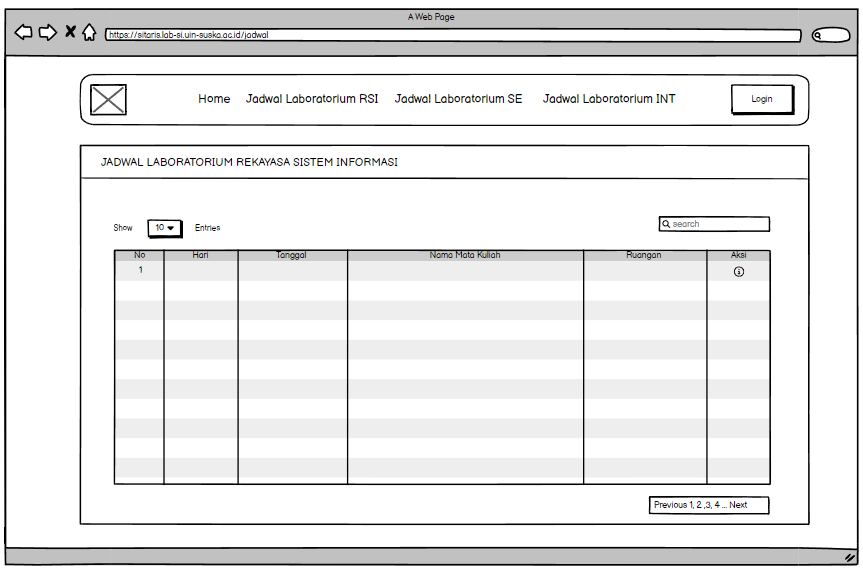
\includegraphics[width=0.82\textwidth]{konten/gambar/user interface/ui-jadwal-rsi.png}
		      \caption{Tampilan Kelola Jadwal Laboratorium}
		      \label{fig:jadwal}
	      \end{figure}
	      \begin{figure}
		      \centering
		      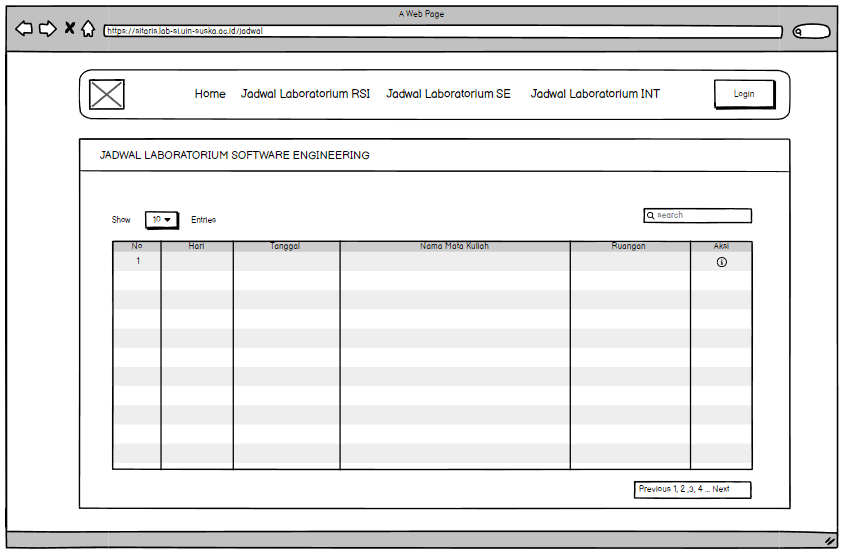
\includegraphics[width=0.82\textwidth]{konten/gambar/user interface/ui-jadwal-se.png}
		      \caption{Tampilan Kelola Jadwal Laboratorium}
		      \label{fig:jadwal}
	      \end{figure}
	      \begin{figure}
		      \centering
		      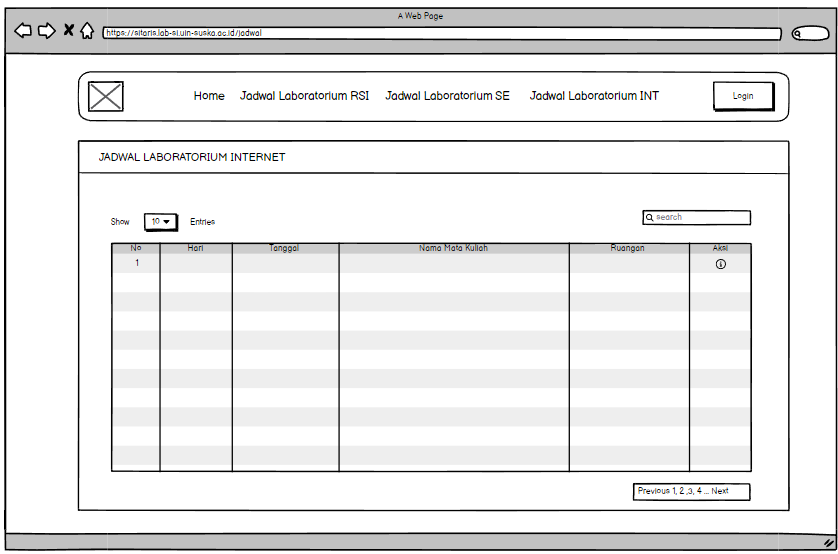
\includegraphics[width=0.82\textwidth]{konten/gambar/user interface/ui-jadwal-int.png}
		      \caption{Tampilan Kelola Jadwal Laboratorium}
		      \label{fig:jadwal}
	      \end{figure}
	\item Rancangan tampilan tambah jadwal yang berfungsi untuk menambah jadwal laboratorium dapat dilihat pada \pic~\ref{fig:jadwal}
	      \begin{figure}
		      \centering
		      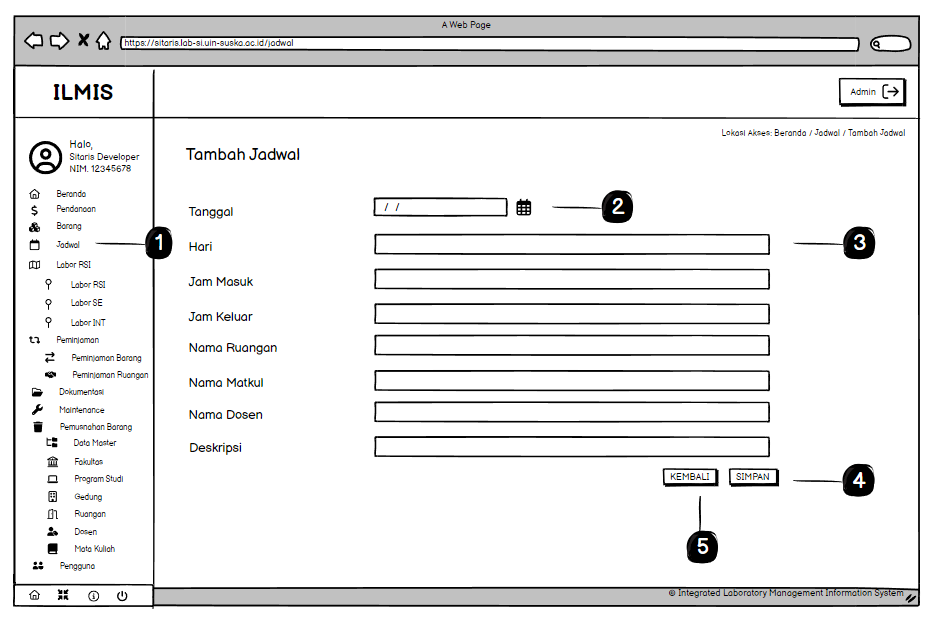
\includegraphics[width=0.82\textwidth]{konten/gambar/tambah-jadwal.png}
		      \caption{Tampilan Tambah Jadwal Laboratorium}
		      \label{fig:jadwal}
	      \end{figure}
	      \begin{table}[H]
		      \centering
		      \caption{Tabel Keterangan Tampilan Tambah Jadwal}
		      \label{tab:tambah-jadwal}
		      \begin{tabular}{|c|p{0.55\textwidth}|}
			      \hline
			      \textbf{Nomor Callouts} & \textbf{Keterangan}                                                                                                                                           \\
			      \hline
			      1                       & Berisi menu navigasi dengan ikon dan teks, menggunakan font-family: Poppins, font-size: 14px. Memiliki warna latar gelap dan ikon menu terorganisir vertikal. \\
			      2                       & Field input untuk memasukkan tanggal dengan placeholder dd/mm/yyyy. Terdapat ikon kalender di sebelah kanan untuk membantu memilih tanggal.                   \\
			      3                       & Berisi beberapa form input untuk memasukkan data berikut:                                                                                                     \\
			                              & - Hari: Input teks untuk memilih atau memasukkan hari.                                                                                                        \\
			                              & - Jam Masuk dan Jam Keluar: Input waktu dengan ikon jam di sebelah kanan.                                                                                     \\
			                              & - Nama Ruangan, Nama Mata Kuliah, dan Nama Dosen: Dropdown untuk memilih opsi.                                                                                \\
			                              & - Deskripsi: Area teks kosong untuk menambahkan keterangan lebih lanjut.                                                                                      \\
			      4                       & Dua tombol aksi:                                                                                                                                              \\
			                              & - Tombol Kembali: Berwarna merah (\#FF5A5F) dengan padding: 12px 24px, border-radius: 6px.                                                                    \\
			                              & - Tombol Simpan: Berwarna biru (\#2563EB) dengan padding: 12px 24px, border-radius: 6px.                                                                      \\
			      5                       & Teks di bagian bawah layar yang menampilkan informasi seperti hak cipta atau detail versi aplikasi. Font-size kecil dengan warna abu-abu muda.                \\
			      \hline
		      \end{tabular}
	      \end{table}

	\item Rancangan tampilan edit jadwal yang berfungsi untuk mengedit jadwal laboratorium dapat dilihat pada \pic~\ref{fig:edit-jadwal}
	      \begin{figure}
		      \centering
		      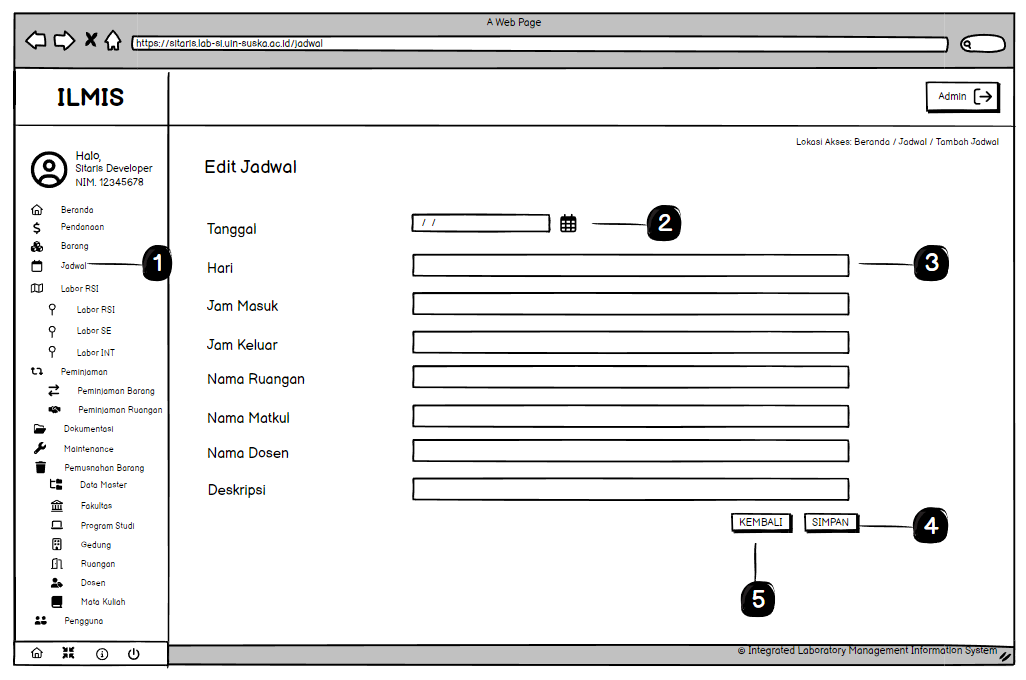
\includegraphics[width=0.82\textwidth]{konten/gambar/user interface/edit-jadwal.png}
		      \caption{Tampilan Edit Jadwal Laboratorium}
		      \label{fig:edit-jadwal}
	      \end{figure}

	      \begin{table}[H]
		      \centering
		      \caption{Tabel Keterangan Tampilan Edit Jadwal}
		      \label{tab:edit-jadwal}
		      \begin{tabular}{|c|p{0.55\textwidth}|}
			      \hline
			      \textbf{Nomor Callouts} & \textbf{Keterangan}                                                                                                                                           \\
			      \hline
			      1                       & Berisi menu navigasi dengan ikon dan teks, menggunakan font-family: Poppins, font-size: 14px. Memiliki warna latar gelap dan ikon menu terorganisir vertikal. \\
			      2                       & Field input untuk memasukkan tanggal dengan placeholder dd/mm/yyyy. Terdapat ikon kalender di sebelah kanan untuk membantu memilih tanggal.                   \\
			      3                       & Berisi beberapa form input untuk memasukkan data berikut:                                                                                                     \\
			                              & - Hari: Input teks untuk memilih atau memasukkan hari.                                                                                                        \\
			                              & - Jam Masuk dan Jam Keluar: Input waktu dengan ikon jam di sebelah kanan.                                                                                     \\
			                              & - Nama Ruangan, Nama Mata Kuliah, dan Nama Dosen: Dropdown untuk memilih opsi.                                                                                \\
			                              & - Deskripsi: Area teks kosong untuk menambahkan keterangan lebih lanjut.                                                                                      \\
			      4                       & Dua tombol aksi:                                                                                                                                              \\
			                              & - Tombol Kembali: Berwarna merah (\#FF5A5F) dengan padding: 12px 24px, border-radius: 6px.                                                                    \\
			                              & - Tombol Simpan: Berwarna biru (\#2563EB) dengan padding: 12px 24px, border-radius: 6px.                                                                      \\
			      5                       & Teks di bagian bawah layar yang menampilkan informasi seperti hak cipta atau detail versi aplikasi. Font-size kecil dengan warna abu-abu muda.                \\
			      \hline
		      \end{tabular}
	      \end{table}

	\item Rancangan tampilan kelola mata kuliah yang berfungsi untuk mengelola mata kuliah laboratorium dapat dilihat pada \pic~\ref{fig:matkul} dan keterangan \textit{user interface} sama dengan \tab~\ref{tab:ui-jadwal}
	      \begin{figure}
		      \centering
		      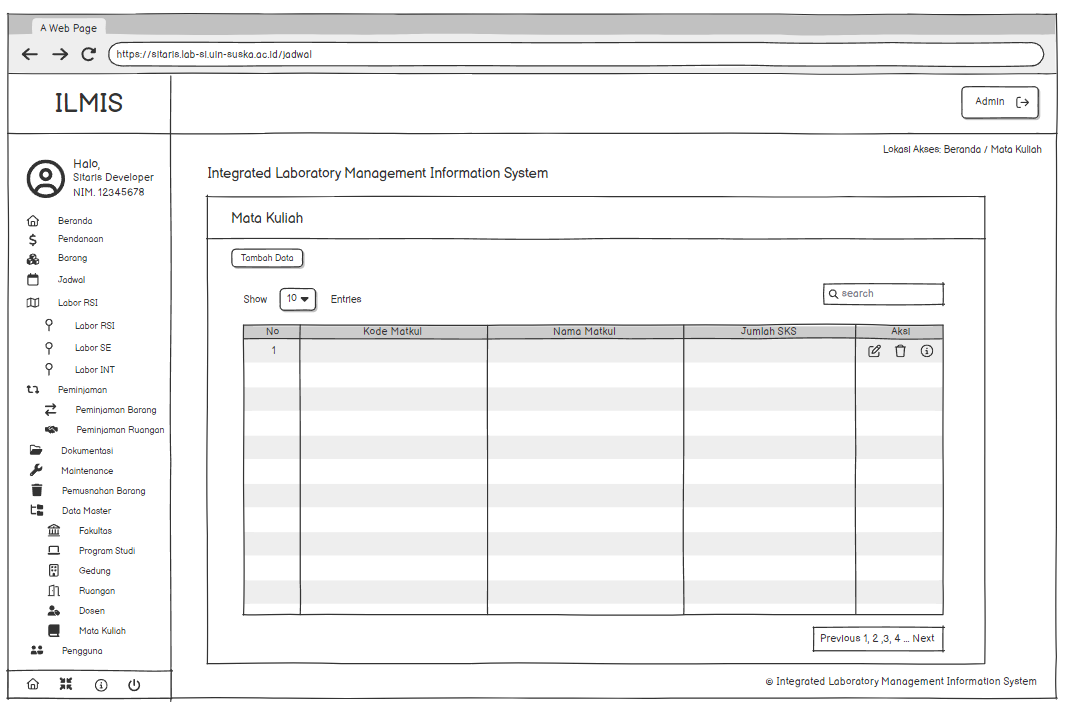
\includegraphics[width=0.82\textwidth]{konten/gambar/user interface/ui-matkul.png}
		      \caption{Tampilan Kelola Mata Kuliah Laboratorium}
		      \label{fig:matkul}
	      \end{figure}
	\item Rancangan tampilan tambah mata kuliah yang berfungsi untuk menambah mata kuliah dapat dilihat pada \pic~\ref{fig:tambah-matkul} dan keterangan \textit{user interface} sama dengan \tab~\ref{tab:tambah-jadwal}
	      \begin{figure}
		      \centering
		      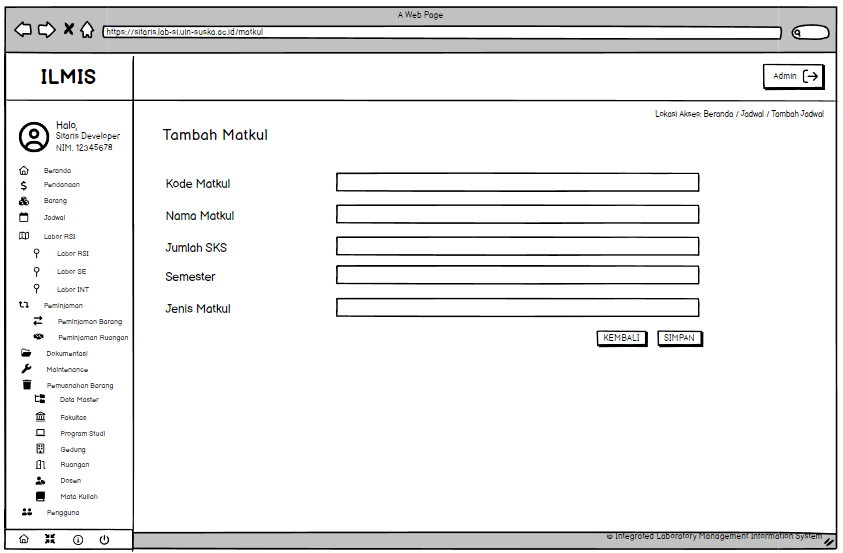
\includegraphics[width=0.82\textwidth]{konten/gambar/user interface/tambah-matkul.png}
		      \caption{Tampilan Tambah Mata Kuliah Laboratorium}
		      \label{fig:tambah-matkul}
	      \end{figure}
	\item Rancangan tampilan edit mata kuliah yang berfungsi untuk mengedit mata kuliah laboratorium dapat dilihat pada \pic~\ref{fig:edit-matkul} dan keterangan \textit{user interface} sama dengan \tab~\ref{tab:edit-jadwal}
	      \begin{figure}
		      \centering
		      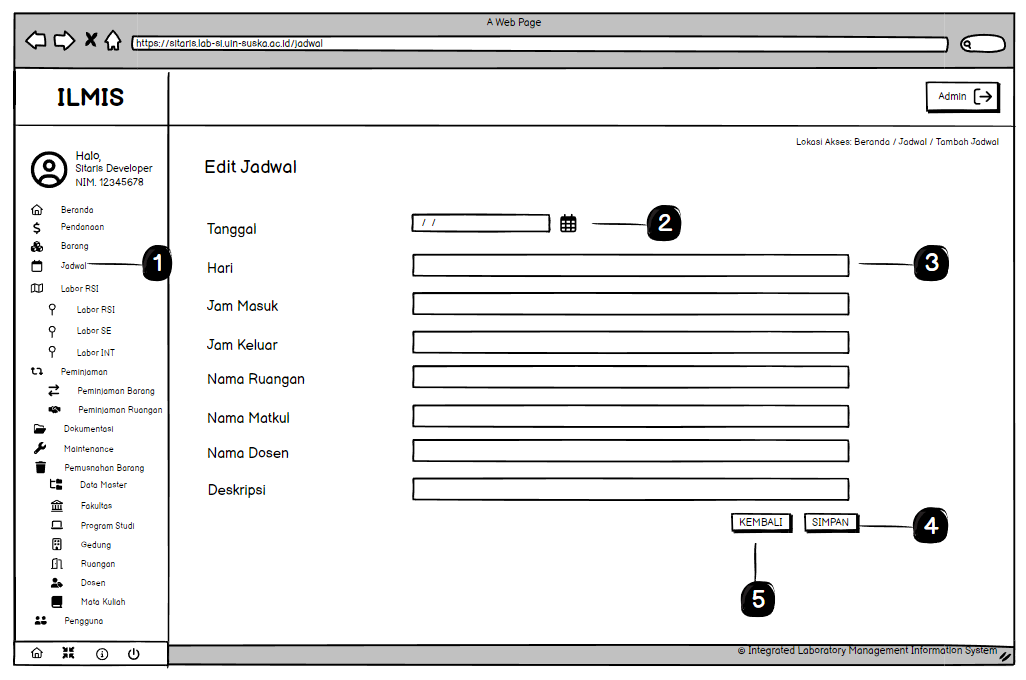
\includegraphics[width=0.82\textwidth]{konten/gambar/user interface/edit-jadwal.png}
		      \caption{Tampilan Edit Mata Kuliah Laboratorium}
		      \label{fig:edit-matkul}
	      \end{figure}
	\item Rancangan tampilan kelola dosen yang berfungsi untuk mengelola dosen laboratorium dapat dilihat pada \pic~\ref{fig:dosen} dan keterangan \textit{user interface} sama dengan \tab~\ref{tab:ui-jadwal}
	      \begin{figure}
		      \centering
		      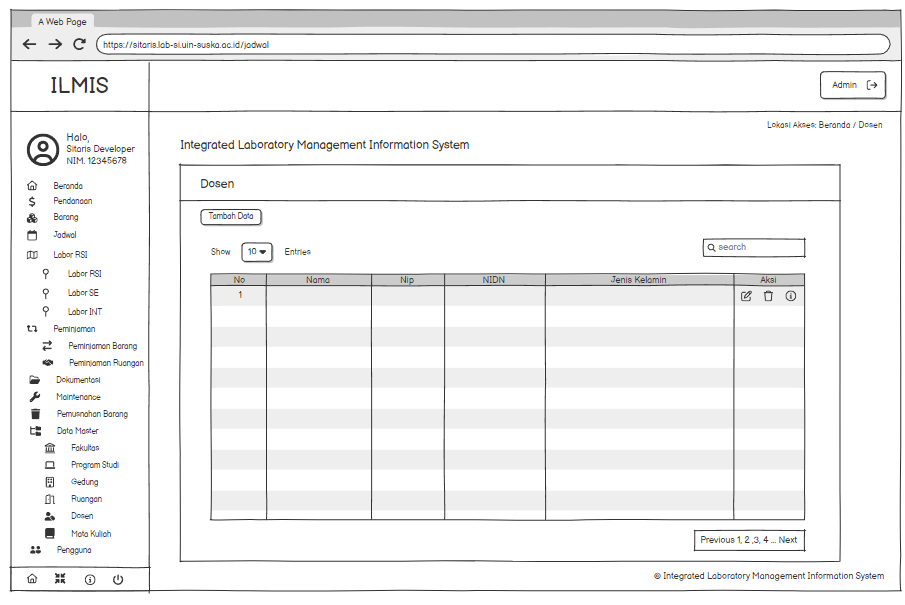
\includegraphics[width=0.82\textwidth]{konten/gambar/user interface/ui-dosen.png}
		      \caption{Tampilan Kelola Dosen Laboratorium}
		      \label{fig:dosen}
	      \end{figure}
	\item Rancangan tampilan tambah dosen yang berfungsi untuk menambah dosen laboratorium dapat dilihat pada \pic~\ref{fig:tambah-dosen} dan keterangan \textit{user interface} sama dengan \tab~\ref{tab:tambah-jadwal}
	      \begin{figure}
		      \centering
		      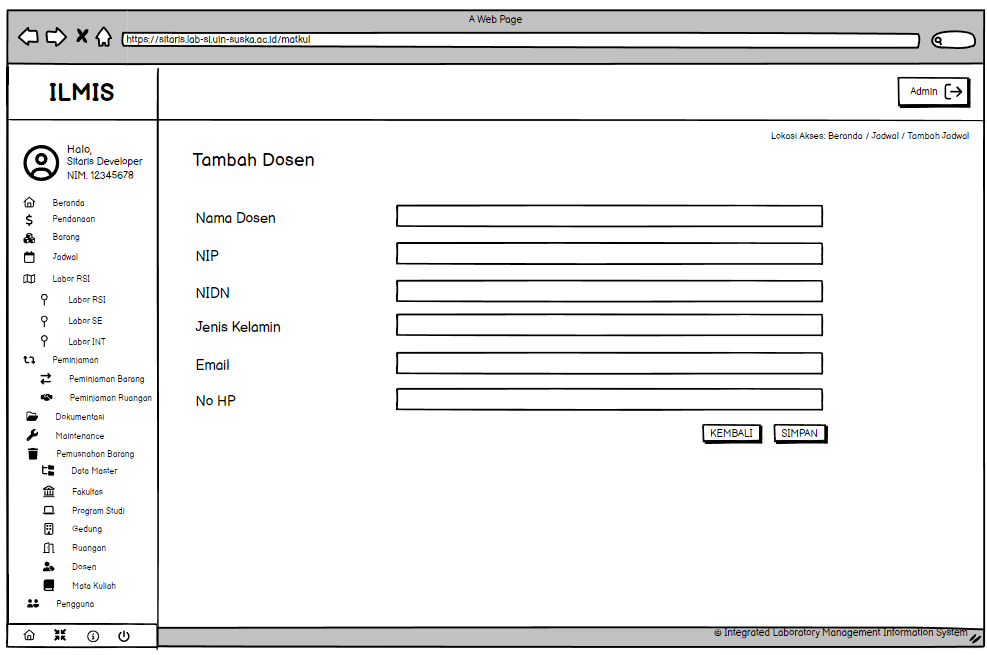
\includegraphics[width=0.82\textwidth]{konten/gambar/user interface/tambah-dosen.png}
		      \caption{Tampilan Tambah Dosen Laboratorium}
		      \label{fig:tambah-dosen}
	      \end{figure}
	\item Rancangan tampilan edit dosen yang berfungsi untuk mengelola dosen laboratorium dapat dilihat pada \pic~\ref{fig:edit-dosen} dan keterangan \textit{user interface} sama dengan \tab~\ref{tab:edit-jadwal}
	      \begin{figure}
		      \centering
		      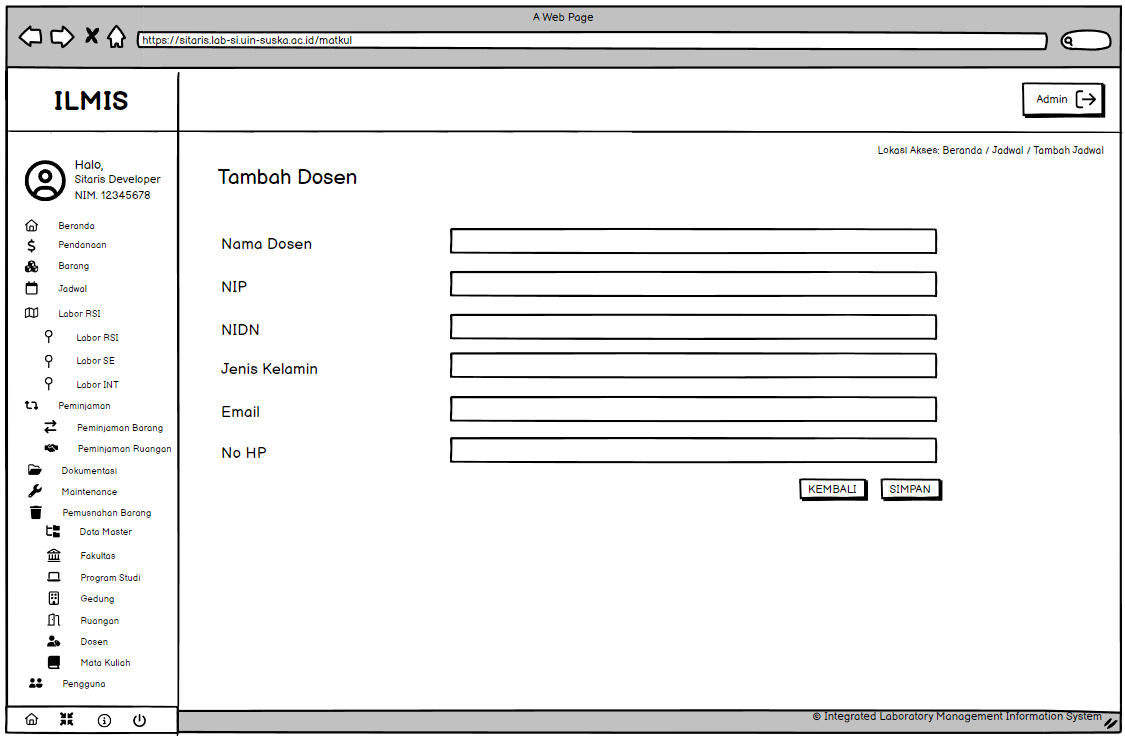
\includegraphics[width=0.82\textwidth]{konten/gambar/user interface/edit-dosen.png}
		      \caption{Tampilan Edit Dosen Laboratorium}
		      \label{fig:edit-dosen}
	      \end{figure}
\end{enumerate}
